\newpage
\section{Mock up}
\subsection*{Introduzione}
Dopo aver definito gli use case utilizzando il metodo Cockburn, siamo passati alla fase di progettazione visiva realizzando una serie di mockup interattivi in Figma. Questi mockup hanno lo scopo di rappresentare graficamente le interazioni dell'utente con il sistema, traducendo le specifiche funzionali in un'interfaccia visibile e navigabile. Ogni mockup è stato sviluppato tenendo conto delle diverse casistiche previste negli use case e nelle loro estensioni, in modo da garantire un’esperienza utente coerente e intuitiva.

Nei paragrafi seguenti verranno presentati i vari mockup, suddivisi per use case. Ogni sezione illustrerà le scelte progettuali effettuate, evidenziando come la UI si adatti alle diverse situazioni previste dai casi d'uso.

\subsection{Caso d'Uso: Aggiungi un Annuncio Immobiliare}

Per garantire un’esperienza utente ottimale, abbiamo progettato i mockup del caso d'uso \textit{Aggiungi un Annuncio Immobiliare} seguendo i principi della user experience (UX) e dell'usabilità. Il percorso utente è stato studiato attentamente per minimizzare il carico cognitivo e semplificare l’interazione, in linea con i modelli proposti da Nielsen e Norman \cite{nielsen1995,norman1988}.

\subsection*{Schermata Iniziale: Gestione Annunci Immobiliari}
L’azione di aggiungere un nuovo annuncio parte dalla schermata di Gestione Annunci Immobiliari, dove l’utente trova:
\begin{itemize}
    \item \textbf{Una lista degli immobili a lui associati}, che consente una rapida contestualizzazione.
    \item \textbf{Un pulsante unico ed evidente}, etichettato “Aggiungi Annuncio Immobiliare”, che centralizza l’azione primaria.
\end{itemize}

\subsection*{Flusso di Navigazione e Segmentazione del Form}
Al click del pulsante, l’utente viene indirizzato a una schermata dedicata alla compilazione di un form articolato in più step. Questa segmentazione si basa sul principio del \textbf{chunking dell’informazione} \cite{miller1956}, riducendo il carico di memoria e rendendo il processo meno gravoso. In particolare:
\begin{itemize}
    \item \textbf{Step 1:} Richiede le informazioni basilari, quali il titolo, il tipo di contratto e il tipo di immobile.
    \item \textbf{Step 2 e successivi:} Raccolgono i dati principali e le caratteristiche secondarie dell’immobile, organizzati in modo logico e intuitivo.
\end{itemize}

\subsection*{Navigazione Sticky e Accessibilità degli Step}
I pulsanti di navigazione, posizionati in alto con comportamento \textit{sticky}, consentono all’utente di passare agevolmente da uno step all’altro, anche in presenza di schermate particolarmente lunghe. Tale scelta:
\begin{itemize}
    \item Riduce il tempo necessario per individuare i controlli di navigazione.
    \item Favorisce un’interazione continua e fluida, in linea con i principi di design centrato sull’utente e le best practice in ambito HCI (Human-Computer Interaction) \cite{shneiderman2004}.
\end{itemize}

\subsection*{Integrazione della Mappa Interattiva}
Per quanto riguarda l’inserimento dell’indirizzo:
\begin{itemize}
    \item \textbf{La mappa interattiva} permette di visualizzare immediatamente la posizione indicata, offrendo un feedback visivo diretto.
    \item L’utente ha la possibilità di regolare la posizione direttamente sulla mappa, migliorando la precisione del dato inserito \cite{wickens2008}.
\end{itemize}

\subsection*{Gestione delle Immagini e Feedback Visivo}
La sezione dedicata alle immagini è progettata per:
\begin{itemize}
    \item \textbf{Consentire l’aggiunta di foto} tramite pulsante dedicato o drag and drop, facilitando l’upload in maniera intuitiva.
    \item \textbf{Permettere l’inserimento di una descrizione} per ogni immagine, migliorando la contestualizzazione visiva dell’annuncio \cite{pieters2004}.
\end{itemize}

\subsection*{Anteprima e Conferma Finale}
Infine, viene presentato uno schema riepilogativo che funge da anteprima dell’annuncio così come apparirà agli utenti finali. Una volta verificata la correttezza dei dati:
\begin{itemize}
    \item L’utente può cliccare il pulsante \textbf{“Pubblica”}, che innesca un processo di caricamento e validazione.
    \item Al termine del processo, viene mostrato un messaggio di conferma che attesta il successo dell’operazione, riducendo l’ansia da incertezza e rafforzando la fiducia nel sistema \cite{nielsen1995}.
\end{itemize}

\newpage

\begin{figure}[ht]
    \centering
    \begin{tikzpicture}[node distance=1.5cm and 1cm, auto]
        % Nodo per immagine 1 con didascalia sotto
        \node (img1) {
            \begin{tabular}{c}
                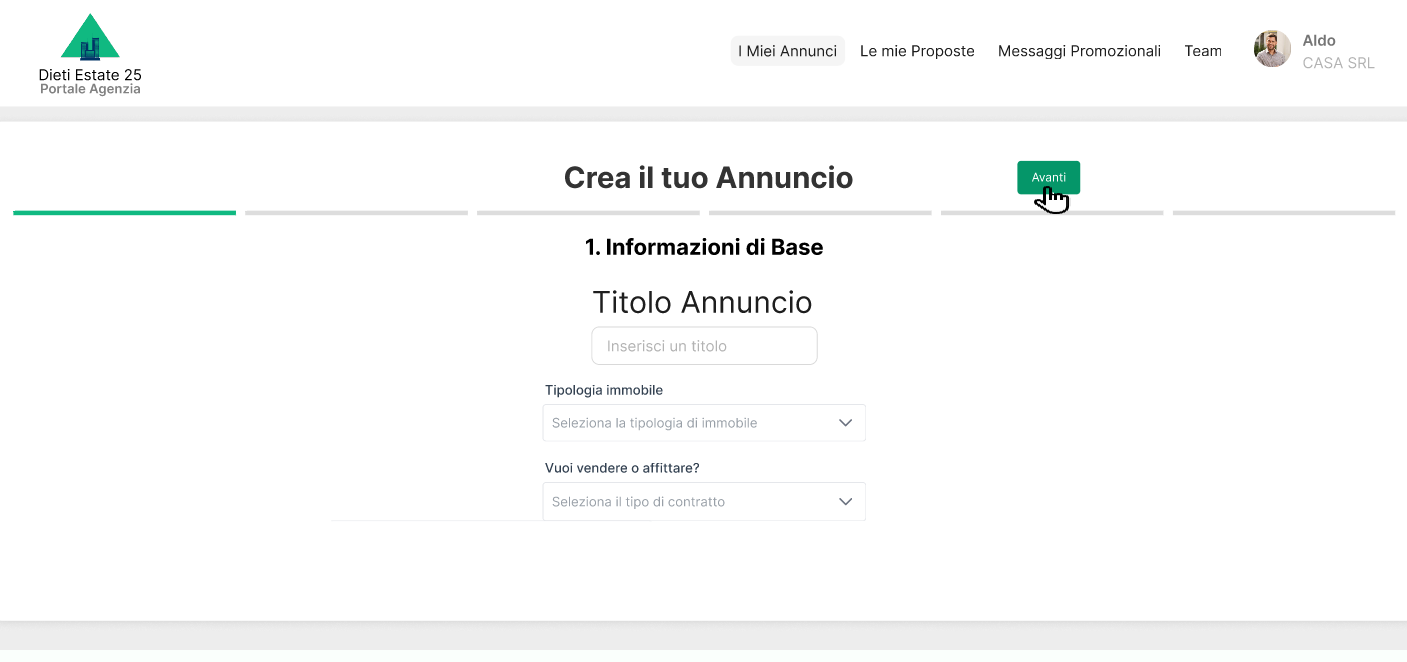
\includegraphics[width=0.7\textwidth]{Immagini/Mockup/aggiungi annuncio/scenario principale/step1.png} \\
                Cockburn: step 3
            \end{tabular}
        };
        
        % Nodo per immagine 2 con didascalia sotto, posizionato a destra di img1
        \node (img2) [below=of img1] {
            \begin{tabular}{c}
                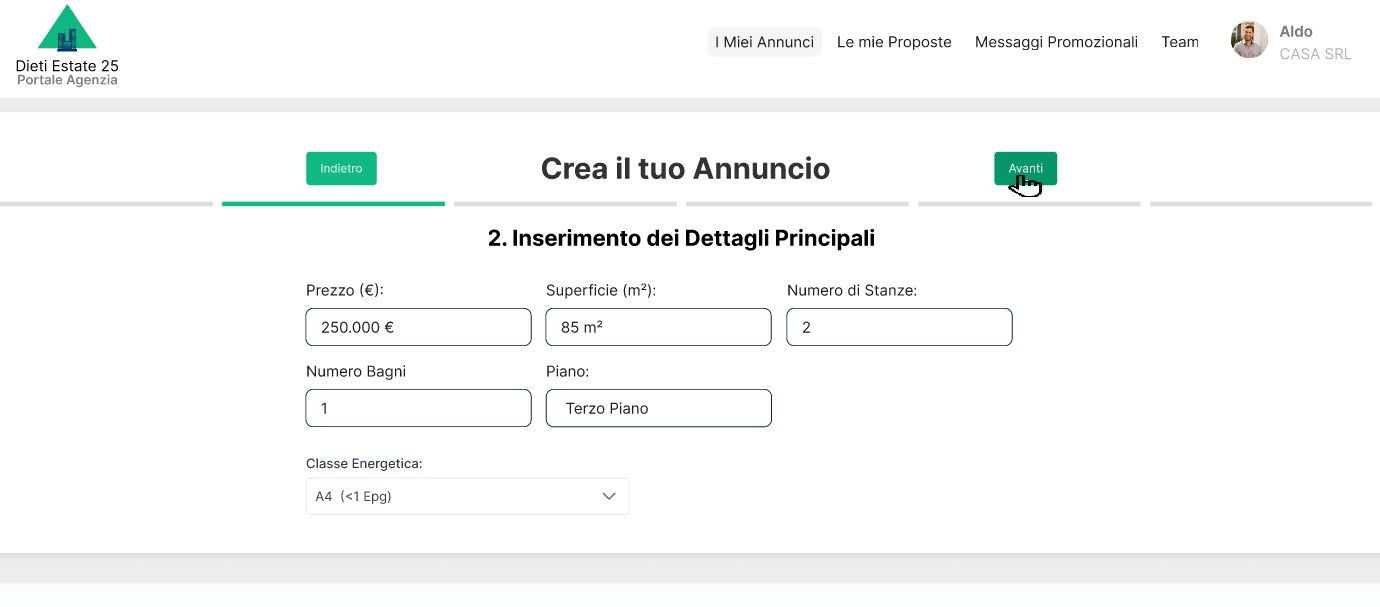
\includegraphics[width=0.7\textwidth]{Immagini/Mockup/aggiungi annuncio/scenario principale/step2.png} \\
                Cockburn: step4/5
            \end{tabular}
        };
        
        % Nodo per immagine 3 con didascalia sotto, posizionato sotto img2
        \node (img3) [below=of img2] {
            \begin{tabular}{c}
                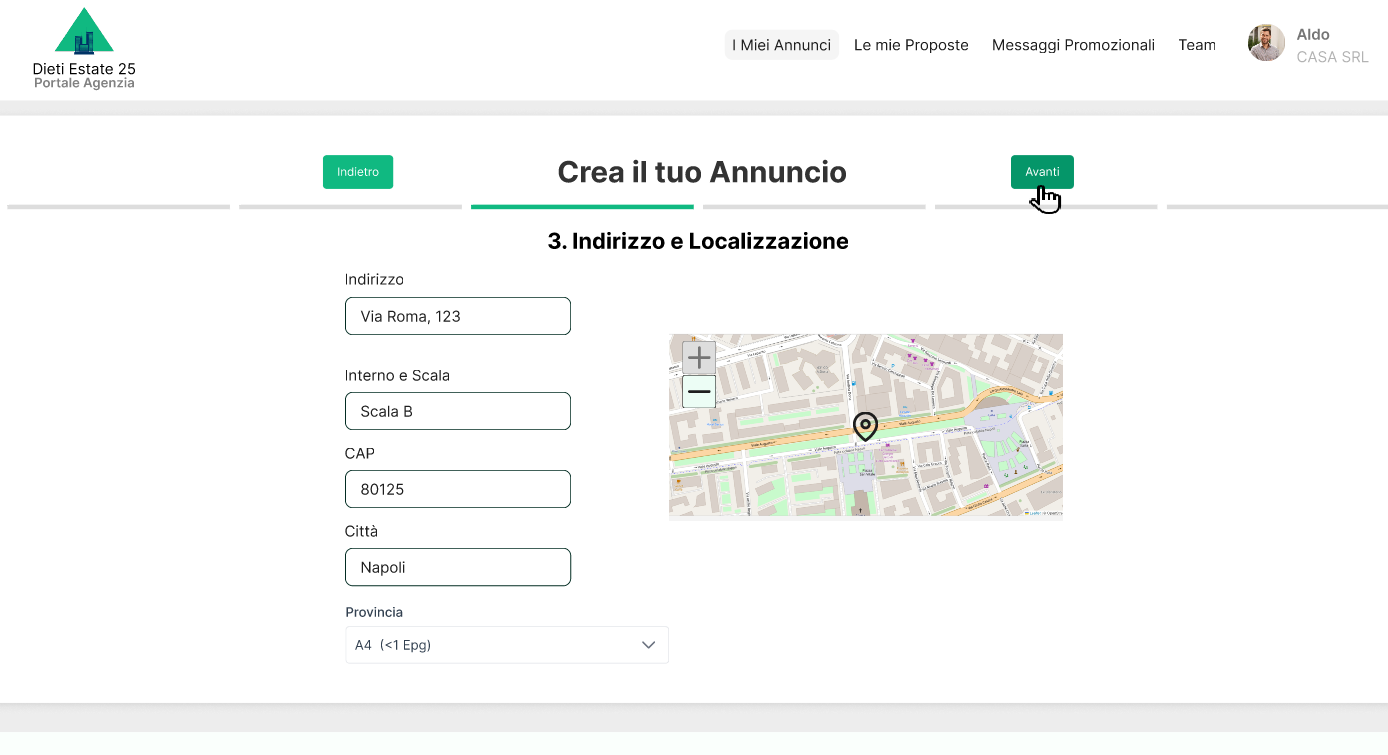
\includegraphics[width=0.7\textwidth]{Immagini/Mockup/aggiungi annuncio/scenario principale/step3.png} \\
                Cockburn: step 4/5
            \end{tabular}
        };
        
        % Disegna le frecce
        \draw[->, thick] (img1) -- (img2);
        \draw[->, thick] (img2) -- (img3);
      
    \end{tikzpicture}
    \caption{Mockup: scenario principale della tabella di Cockburn del caso d'uso nuovo annuncio.}
    \label{fig:mockup_scenario_principale_parte1_aggiungi_annuncio}
\end{figure}

\newpage



\begin{figure}[ht]
    \centering
    \begin{tikzpicture}[node distance=1.5cm and 1cm, auto]
        % Nodo per immagine 1 con didascalia sotto
        \node (img1) {
            \begin{tabular}{c}
                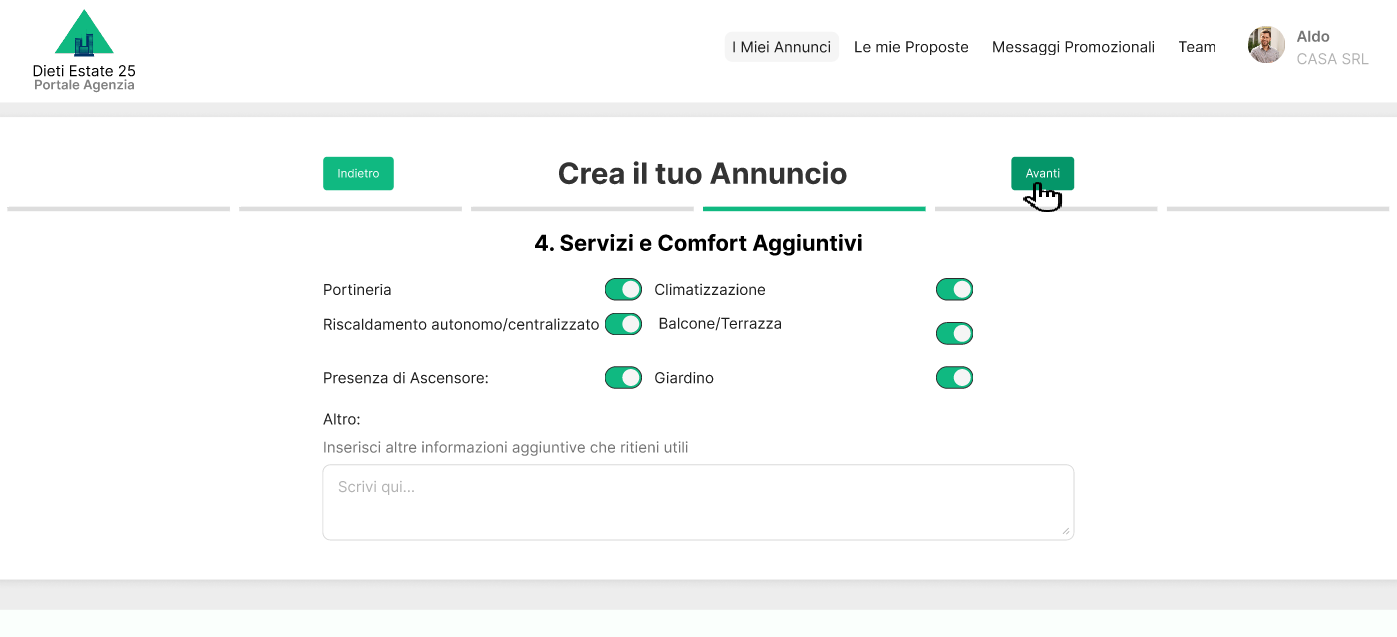
\includegraphics[width=\textwidth,keepaspectratio]{Immagini/Mockup/aggiungi annuncio/scenario principale/step4.png} \\
                Cockburn: step 4/5
            \end{tabular}
        };
        
        % Nodo per immagine 2 con didascalia sotto, posizionato a destra di img1
        \node (img2) [below=of img1] {
            \begin{tabular}{c}
                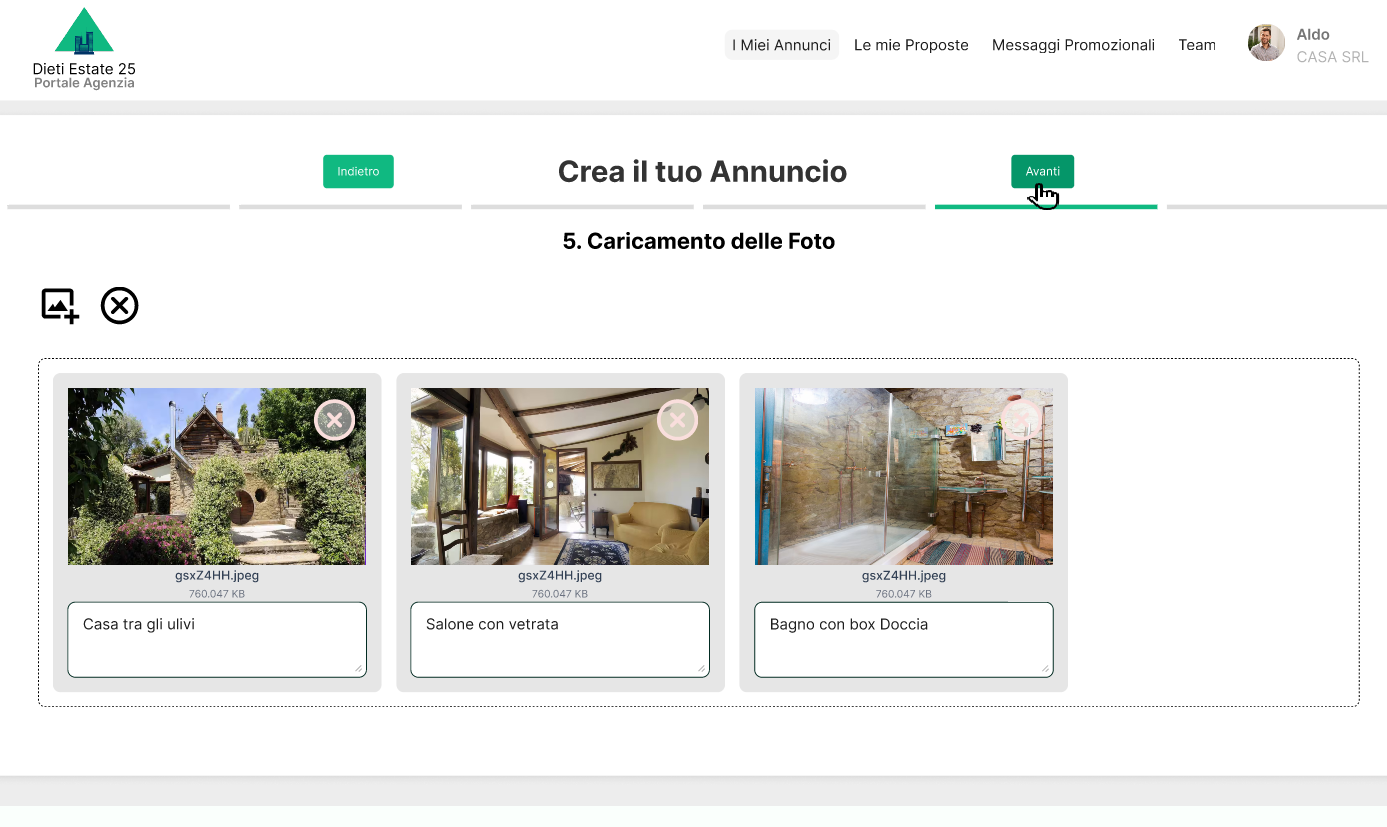
\includegraphics[width=\textwidth,keepaspectratio]{Immagini/Mockup/aggiungi annuncio/scenario principale/step5.png} \\
                Cockburn: step 6
            \end{tabular}
        };
        
        % Disegna le frecce
        \draw[->, thick] (img1) -- (img2);
      
    \end{tikzpicture}
    \caption{Mockup: scenario principale della tabella di Cockburn del caso d'uso nuovo annuncio.}
    \label{fig:tikz_flow}
\end{figure}

\newpage

\input{Requisiti Del Software/Analisi dei Requisiti/Mockup/aggiungi annuncio/scenario principale Parte III}



\clearpage
\newpage

\subsubsection{Estensione A: Disattivazione Notifiche dalla Visualizzazione di una Notifica}

Per offrire un maggiore controllo sulla gestione delle notifiche senza interrompere l’esperienza utente, il sistema permette di disattivare una categoria direttamente dalla visualizzazione di una notifica specifica. Questa variante è progettata per garantire una modifica consapevole delle preferenze, evitando azioni impulsive che potrebbero compromettere la ricezione di informazioni rilevanti.

\vspace{0.5cm}
\subsubsection{Interfaccia e Comportamento del Bottone}
Alla fine del testo di ogni notifica, se la relativa categoria è attiva, è presente un pulsante neutro con la dicitura “Disattiva notifiche”. Accanto al pulsante, un testo in grigio informa l’utente della funzione del pulsante, evitando ambiguità. L’utilizzo di colori non accesi e di un design discreto segue il principio della \textbf{gerarchia visiva} \cite{pieters2004}, scoraggiando azioni impulsive che potrebbero portare alla perdita involontaria di notifiche future.

\vspace{0.5cm}
\subsubsection{Modifica dello Stato e Feedback Visivo}
Quando l’utente clicca sul pulsante, il testo del pulsante cambia colore, diventando rosso, e il messaggio a fianco si aggiorna per sottolineare che la categoria di notifiche è stata disattivata. Questo utilizza il principio della \textbf{salienza visiva} \cite{nielsen1995}, enfatizzando il cambiamento e rendendo immediatamente chiara la conseguenza dell’azione.

\vspace{0.5cm}
\subsubsection{Incentivo alla Riattivazione}
Una volta disattivata una categoria tramite questa modalità, viene visualizzato un secondo pulsante con una call-to-action mirata per incentivare la riattivazione delle notifiche. Il design e il posizionamento del pulsante sfruttano il \textbf{principio dell’affordance} \cite{norman1988}, rendendo chiaro che l’utente ha la possibilità di tornare indietro sulla sua decisione in modo semplice e immediato.
\newline
Questa estensione si integra perfettamente con il modello generale di gestione delle notifiche, garantendo un’interazione fluida e coerente con le esigenze dell’utente. Nel caso in cui l’utente scelga di riattivare la categoria delle notifiche direttamente da una notifica, si passa all’\textbf{Estensione F}, che approfondisce questa modalità di gestione a partire dalle notifiche disattivate.
\begin{figure}[ht]
    \centering
    \begin{tikzpicture}[node distance=1.5cm and 1cm, auto]
        % Nodo per immagine 1 con didascalia sotto
        \node (img1) {
            \begin{tabular}{c}
                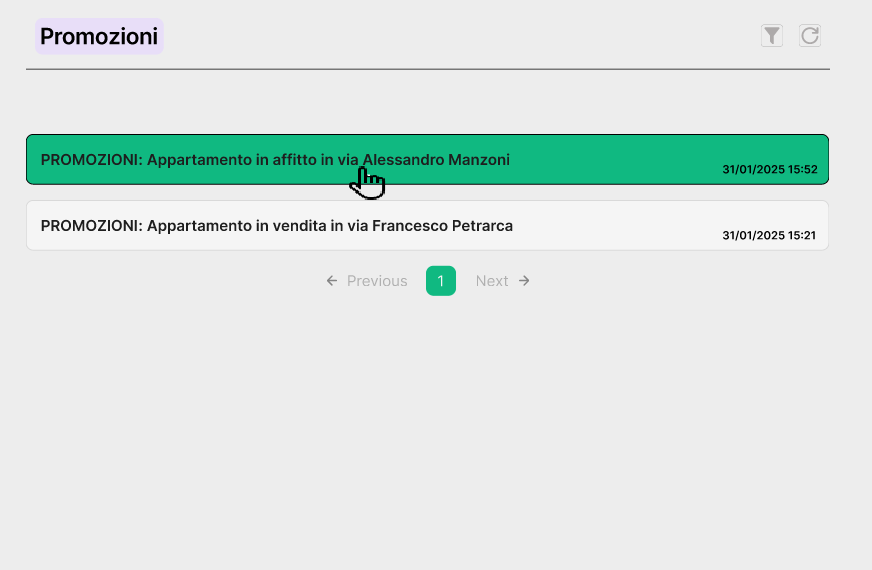
\includegraphics[width=0.4\textwidth]{Immagini/Mockup/notifiche/estensione A/clickNotifica.png} \\
                Cockburn: Extension A.2/A.3
            \end{tabular}
        };
        
        % Nodo per immagine 2 con didascalia sotto, posizionato a destra di img1
        \node (img2) [below=of img1] {
            \begin{tabular}{c}
                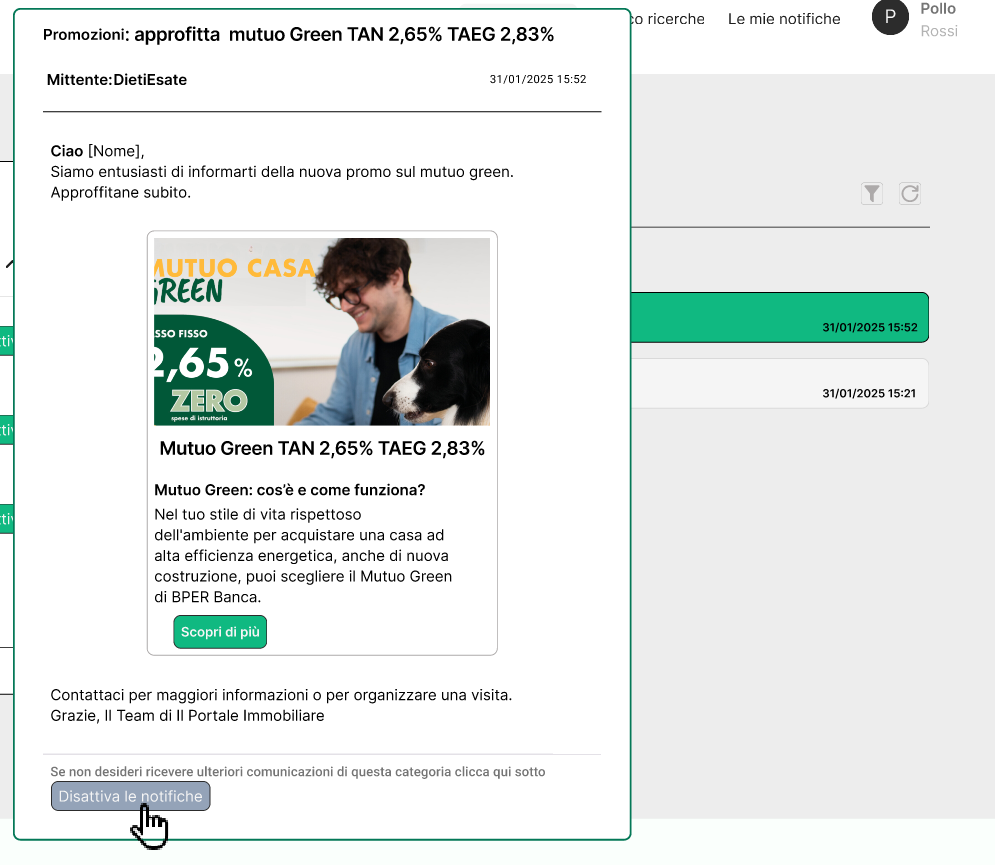
\includegraphics[width=0.4\textwidth]{Immagini/Mockup/notifiche/estensione A/clickDisattiva.png} \\
                Cockburn: Extension A.4
            \end{tabular}
        };
        
        % Nodo per immagine 3 con didascalia sotto, posizionato sotto img2
        \node (img3) [below=of img2] {
            \begin{tabular}{c}
                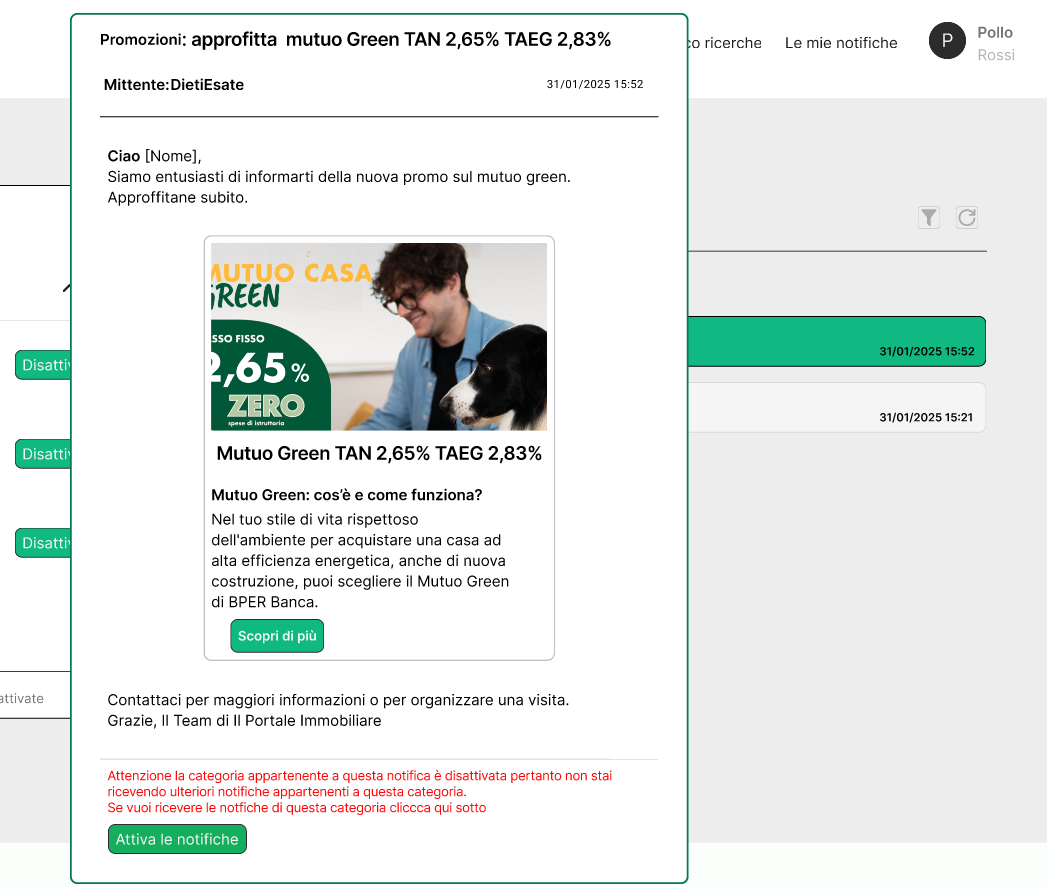
\includegraphics[width=0.4\textwidth]{Immagini/Mockup/notifiche/estensione A/disattivato.png} \\
                Cockburn: extension A.5
            \end{tabular}
        };
        
        % Disegna le frecce
        \draw[->, thick] (img1) -- (img2);
        \draw[->, thick] (img2) -- (img3);
      
    \end{tikzpicture}
    \caption{Mockup: estensione A della tabella di Cockburn del caso d'uso disattiva/attiva categoria notifica}
    \label{fig:mockup_estensione_A_disattiva_notifiche}
\end{figure}

\newpage



\clearpage
\newpage
\subsubsection{Estensione B: Ripristino di un Annuncio Precedente}
Se l’utente sceglie di \textbf{ripristinare l’annuncio precedente}, il sistema avvia un processo di caricamento per fornire un feedback visivo sulla ripresa dei dati. Sebbene i dati siano salvati localmente e il recupero sia immediato, un \textbf{indicatore di caricamento fittizio} viene mostrato per alcuni secondi prima di caricare la schermata.

Questa soluzione è basata sul principio della \textbf{coerenza con le aspettative dell’utente} \cite{shneiderman2004}. In un contesto digitale, un ripristino istantaneo potrebbe apparire innaturale e creare confusione. L’indicatore di caricamento:
\begin{itemize}
    \item Rafforza la percezione di un processo in corso, migliorando la trasparenza dell’operazione.
    \item Evita che l’utente si domandi se il recupero sia realmente avvenuto o se ci siano stati problemi tecnici.
    \item Contribuisce a una transizione più fluida tra stati dell’interfaccia.
\end{itemize}

Una volta completato il caricamento, il sistema presenta l’interfaccia con i dati precedentemente salvati, consentendo all’utente di riprendere il processo da dove era stato interrotto.


\begin{figure}[ht]
    \centering
    \begin{tikzpicture}[node distance=1.5cm and 1cm, auto]
        % Nodo per immagine 1 con didascalia sotto
        \node (img1) {
            \begin{tabular}{c}
                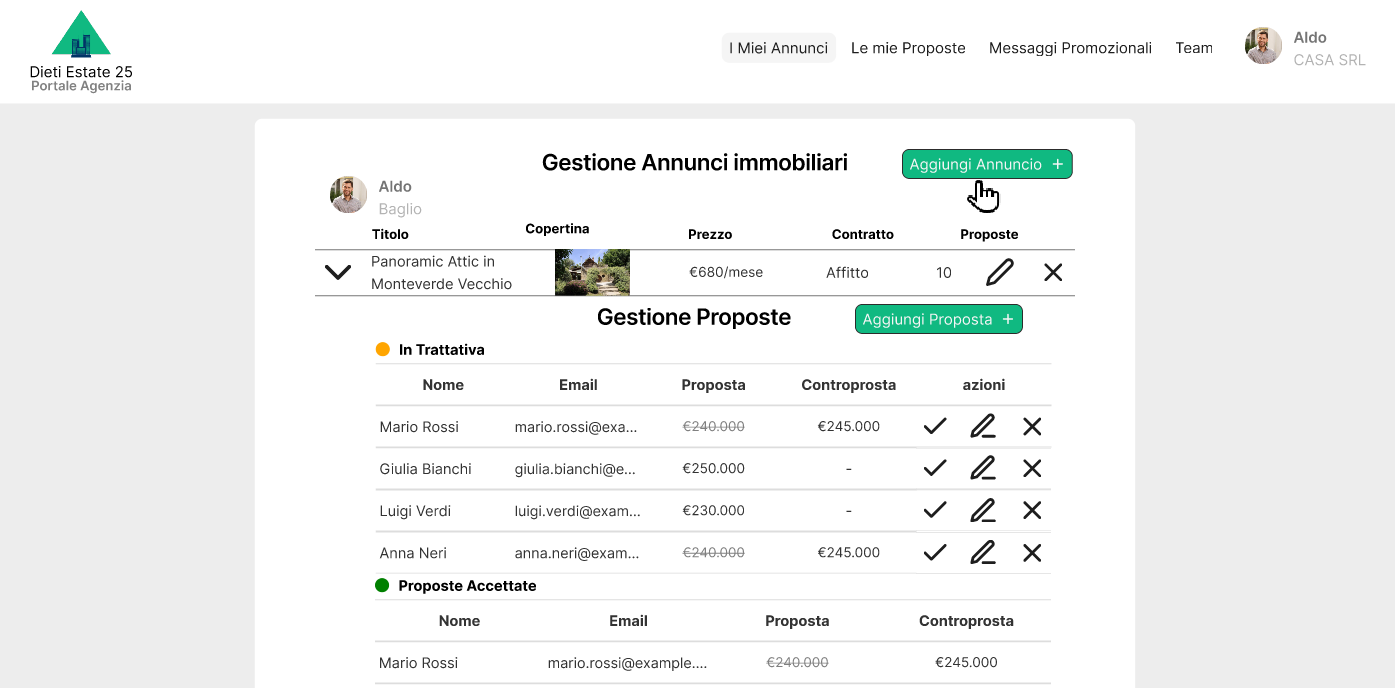
\includegraphics[width=0.7\textwidth]{Immagini/Mockup/aggiungi annuncio/estensione B/step1.png} \\
                click nuovo annuncio
            \end{tabular}
        };
        
        % Nodo per immagine 2 con didascalia sotto, posizionato a destra di img1
        \node (img2) [below=of img1] {
            \begin{tabular}{c}
                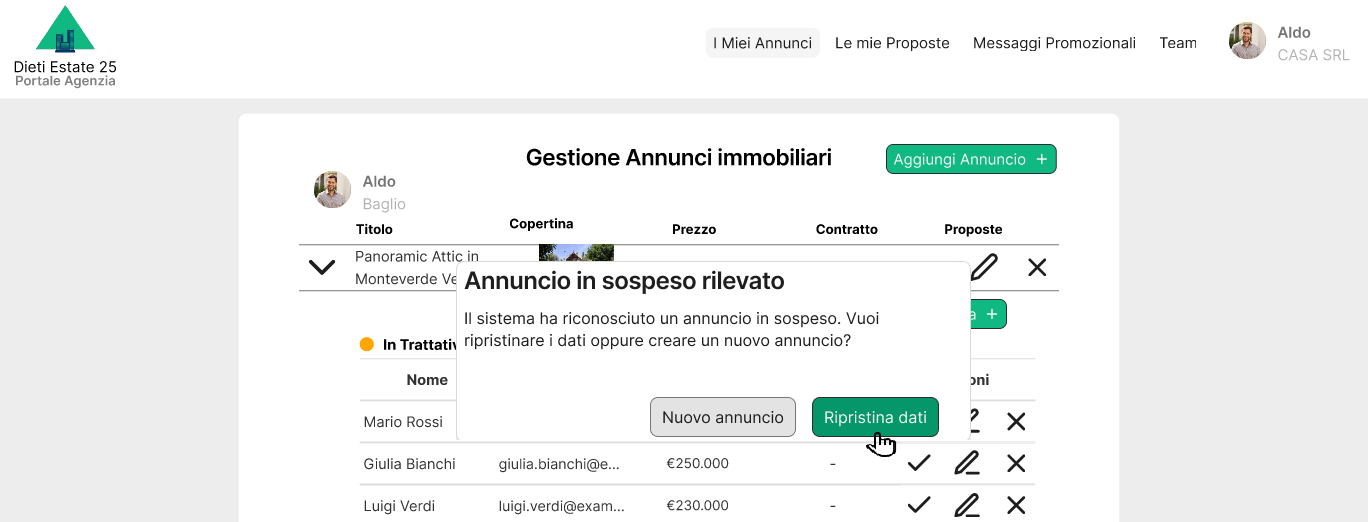
\includegraphics[width=0.7\textwidth]{Immagini/Mockup/aggiungi annuncio/estensione B/step2.png} \\
                Cockburn: extension B.2/B.3/B.4
            \end{tabular}
        };
        
        % Nodo per immagine 3 con didascalia sotto, posizionato sotto img2
        \node (img3) [below=of img2] {
            \begin{tabular}{c}
                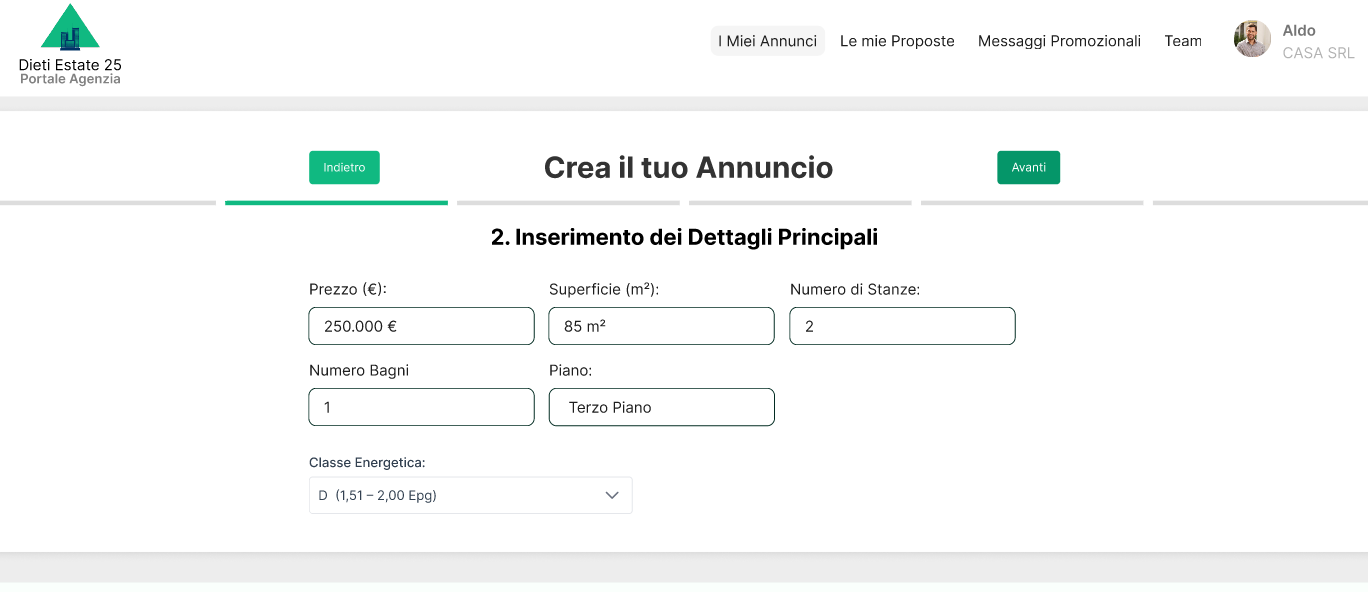
\includegraphics[width=0.7\textwidth]{Immagini/Mockup/aggiungi annuncio/estensione B/step3.png} \\
                Cockburn: extension B.5
            \end{tabular}
        };
        
        % Disegna le frecce
        \draw[->, thick] (img1) -- (img2);
        \draw[->, thick] (img2) -- (img3);
      
    \end{tikzpicture}
    \caption{Mockup: estensione B della tabella di Cockburn del caso d'uso nuovo annuncio}
    \label{fig:mockup_estensione_B_aggiungi_annuncio}
\end{figure}

\newpage




\clearpage
\newpage
\subsubsection{Estensione C: Errore Durante la Pubblicazione dell'Annuncio}

Nel caso in cui si verifichi un errore durante la pubblicazione dell'annuncio immobiliare, viene mostrato un popup informativo che comunica all'utente il problema riscontrato. Questo popup ha il compito di rassicurare l'utente che i dati inseriti non andranno persi, in quanto vengono salvati localmente, e invita a riprovare più tardi.

\subsubsection{Gestione dell'Errore e Feedback Utente}
Il popup presenta i seguenti elementi chiave:
\begin{itemize}
    \item \textbf{Messaggio chiaro e rassicurante}: informa l'utente dell'errore senza tecnicismi, riducendo il senso di frustrazione.
    \item \textbf{Pulsante “Riprova”}: consente di tentare nuovamente la pubblicazione con un'animazione di caricamento, per segnalare che l'azione è in corso e mantenere un senso di controllo e progressione.
    \item \textbf{Pulsante “Monstra i Dettagli”}: offre la possibilità di visualizzare l'errore tecnico riscontrato. Questa funzione segue i principi di trasparenza e controllo dell'utente, utili sia per utenti avanzati che per eventuali tecnici di supporto che potrebbero risolvere il problema più rapidamente.
\end{itemize}

\subsubsection{Principi di Design Applicati}
L'implementazione di questa gestione degli errori si basa su diversi principi della UX e dell'usabilità:
\begin{itemize}
    \item \textbf{Visibilità dello stato del sistema} \cite{nielsen1995}: l'animazione di caricamento fornisce un'indicazione chiara che il sistema sta lavorando sulla richiesta dell'utente.
    \item \textbf{Prevenzione degli errori} \cite{nielsen1995}: il salvataggio locale dei dati riduce la possibilità di perdere informazioni a causa di un problema temporaneo.
    \item \textbf{Fornire informazioni utili per il recupero dall'errore} \cite{nielsen1995}: il messaggio di errore è accompagnato da suggerimenti su come procedere e un'opzione per visualizzare i dettagli tecnici, utile per il supporto tecnico.
\end{itemize}

Queste soluzioni mirano a mantenere un'esperienza utente fluida e priva di frustrazione, minimizzando il disagio derivante da problemi tecnici imprevisti.


\begin{figure}[ht]
    \centering
    \begin{tikzpicture}[node distance=1.5cm and 1cm, auto]
        % Nodo per immagine 1 con didascalia sotto
        \node (img1) {
            \begin{tabular}{c}
                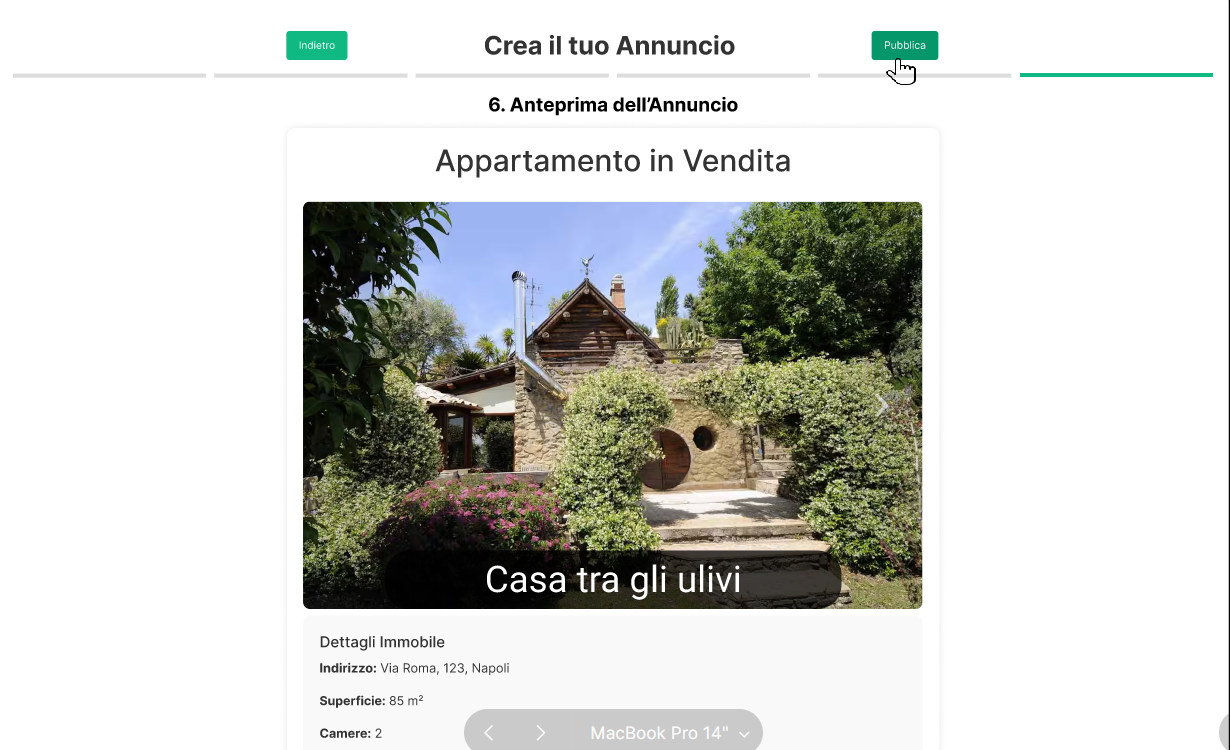
\includegraphics[width=0.7\textwidth]{Immagini/Mockup/aggiungi annuncio/estensione C/step1.png} \\
                click pubblica nuovo annuncio
            \end{tabular}
        };
        
        % Nodo per immagine 2 con didascalia sotto, posizionato a destra di img1
        \node (img2) [below=of img1] {
            \begin{tabular}{c}
                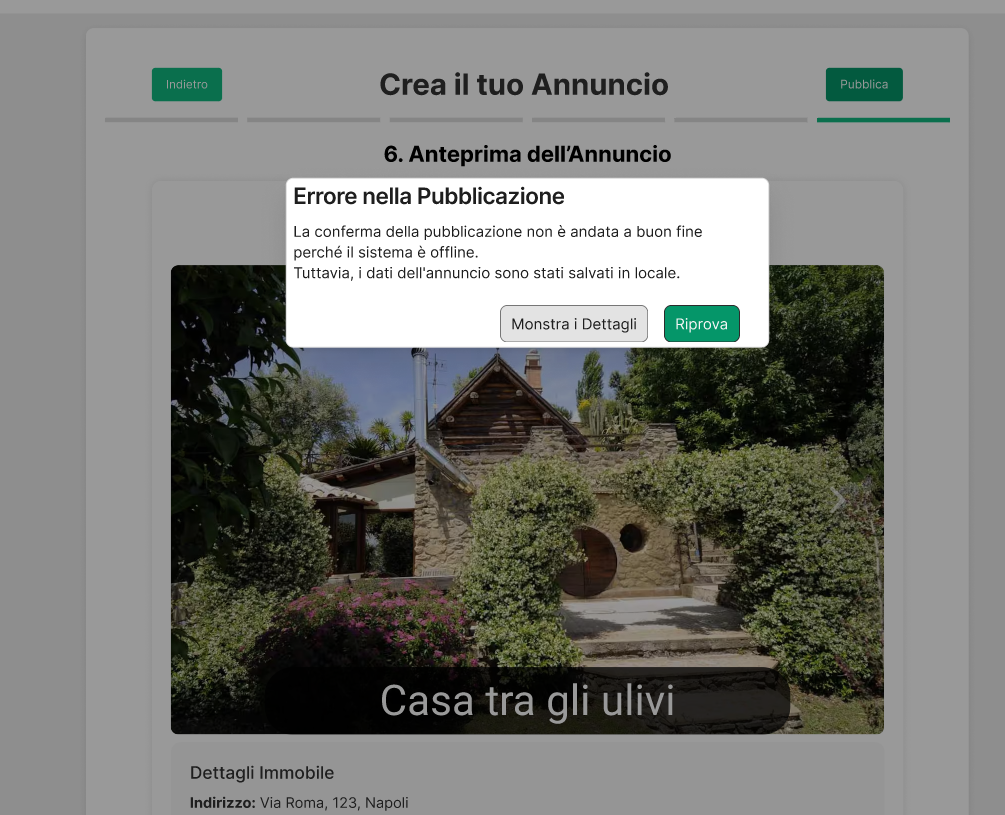
\includegraphics[width=\textwidth]{Immagini/Mockup/aggiungi annuncio/estensione C/step2.png} \\
                Cockburn: extension C.9/C.10
            \end{tabular}
        };
        
        
        % Disegna le frecce
        \draw[->, thick] (img1) -- (img2);
      
    \end{tikzpicture}
    \caption{Mockup: estensione C della tabella di Cockburn del caso d'uso nuovo annuncio}
    \label{fig:tikz_flow}
\end{figure}

\newpage



\clearpage
\newpage

\subsubsection{Estensione D: Modifica Rapida dello Stato delle Notifiche con Attivazione Immediata}

Questa variante rappresenta l’approccio duale dell’\textbf{Estensione C}, semplificando ulteriormente l’attivazione delle notifiche. L’obiettivo è ridurre i passaggi necessari per riattivare una categoria disattivata, mantenendo comunque un controllo chiaro sulla disattivazione.

\vspace{0.5cm}
\subsubsection{Interfaccia e Interazione}
Analogamente all’\textbf{Estensione C}, ogni categoria nella barra laterale dispone di un pulsante contestuale per modificarne lo stato. Il pulsante può assumere due stati:

\begin{itemize}
    \item \textbf{Attiva}, se la categoria è attualmente disabilitata.
    \item \textbf{Disattiva}, se la categoria è attualmente abilitata.
\end{itemize}

Le interazioni dell’utente variano a seconda dell’azione eseguita:

\begin{itemize}
    \item \textbf{Disattivazione di una categoria}:
    \begin{itemize}
        \item Al clic su \textbf{Disattiva}, appare un popup di conferma che informa l’utente sulle conseguenze della scelta, prevenendo azioni accidentali in linea con i principi di Nielsen \cite{nielsen1995}.
        \item Se confermata, la categoria viene spostata nella sezione delle notifiche disattivate tramite un’animazione di transizione.
        \item Il pulsante cambia stato, diventando \textbf{Attiva}, fornendo un feedback visivo chiaro sulla modifica.
    \end{itemize}
    
    \item \textbf{Attivazione di una categoria}:
    \begin{itemize}
        \item Al clic su \textbf{Attiva}, il sistema aggiorna immediatamente lo stato della notifica senza richiedere una conferma esplicita.
        \item La categoria viene spostata nella sezione delle notifiche attive con un’animazione fluida, applicando il principio della \textbf{gestalt della continuità} \cite{miller1956}.
        \item Il pulsante cambia stato in \textbf{Disattiva}, rendendo la modifica evidente e intuitiva.
    \end{itemize}
\end{itemize}

\subsubsection{Feedback Visivo e UX Design}
L’esperienza utente è ottimizzata tramite tecniche di design che garantiscono chiarezza e immediatezza:

\begin{itemize}
    \item \textbf{Popup di conferma per la disattivazione}: aiuta a prevenire errori e rende consapevole l’utente delle conseguenze della scelta \cite{nielsen1995}.
    \item \textbf{Animazione di transizione}: assicura una continuità visiva fluida nello spostamento delle categorie, migliorando la percezione del cambiamento \cite{miller1956}.
    \item \textbf{Aggiornamento immediato dello stato del pulsante}: il cambio di testo e colore riflette lo stato corrente della categoria, riducendo l’ambiguità e migliorando la prevedibilità dell’interazione.
\end{itemize}

Questa estensione semplifica l’attivazione delle notifiche, eliminando il passaggio della conferma e migliorando la fluidità dell’interazione, senza compromettere il controllo dell’utente sulla gestione delle proprie preferenze.

\begin{figure}[ht]
    \centering
    \begin{tikzpicture}[node distance=1.5cm and 1cm, auto]
        % Nodo per immagine 1 con didascalia sotto
        \node (img1) {
            \begin{tabular}{c}
                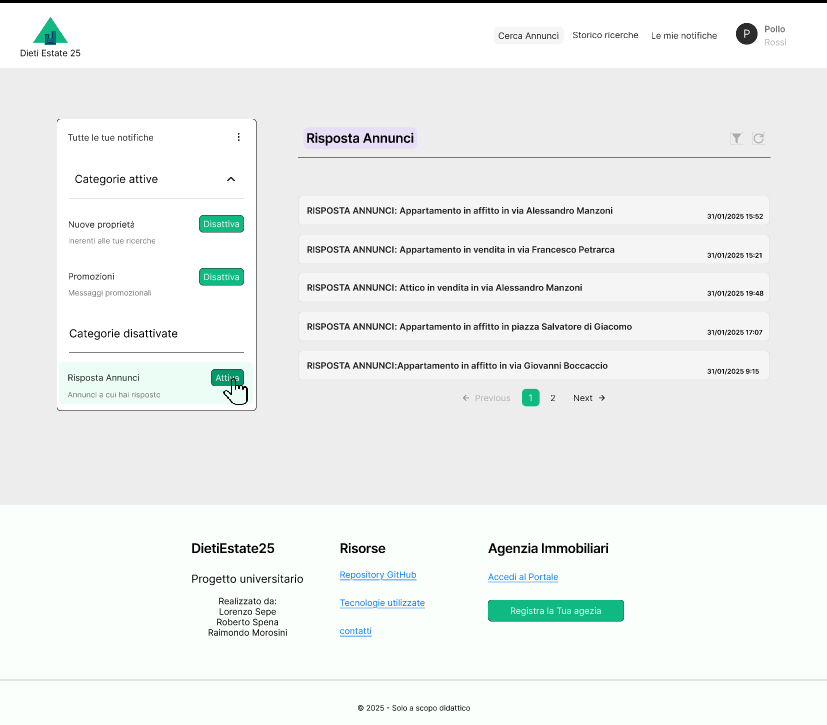
\includegraphics[width=0.6\textwidth]{Immagini/Mockup/notifiche/estensione D/clickAttiva.png} \\
                Cockburn: Extension D.2
            \end{tabular}
        };
        
        % Nodo per immagine 2 con didascalia sotto, posizionato a destra di img1
        \node (img2) [below=of img1] {
            \begin{tabular}{c}
                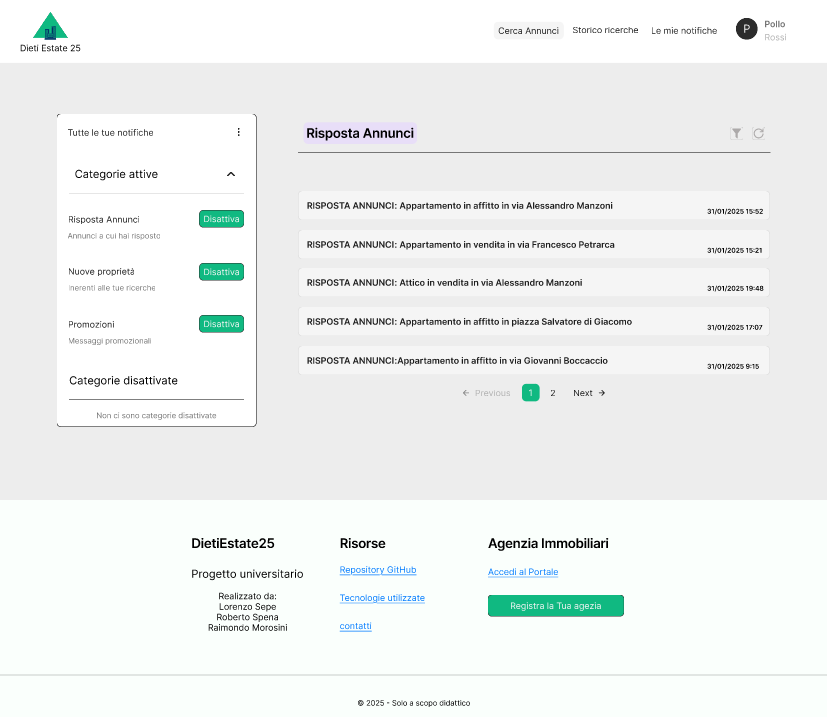
\includegraphics[width=0.6\textwidth]{Immagini/Mockup/notifiche/estensione D/attivato.png} \\
                Cockburn: step 8/9/10
            \end{tabular}
        };
        
        % Disegna le frecce
        \draw[->, thick] (img1) -- (img2);
      
    \end{tikzpicture}
    \caption{Mockup: estensione D della tabella di Cockburn del caso d'uso disattiva/attiva categoria notifica}
    \label{fig:mockup_estensione_D_disattiva_notifiche}
\end{figure}

\newpage



\clearpage
\newpage

\subsection{Caso d'Uso: Attivazione e Disattivazione Notifiche}

Il sistema prevede un'interfaccia dedicata alla gestione delle preferenze di notifica, pensata per permettere all'utente di curare la propria esperienza d'uso dell'applicazione, ricevendo news solo sugli argomenti di interesse.\\
In questa sezione andremo a esaminare le scelte effettuate durante la progettazione, l'impatto sull'esperienza utente e i prototipi generati alla fine dell'analisi. 

\vspace{0.5cm}
\subsubsection{Tipologie di Notifiche e Controllo Utente}
Le notifiche sono suddivise in diverse categorie per permettere una personalizzazione granulare:
\begin{itemize}
    \item \textbf{Annunci di nuovi immobili}: notifiche basate sulle ricerche dell’utente.
    \item \textbf{Risposte alle offerte}: aggiornamenti sulle interazioni con gli annunci pubblicati.
    \item \textbf{Messaggi promozionali}: comunicazioni di marketing e offerte esclusive.
\end{itemize}
L’utente può, in qualsiasi momento, disattivare le notifiche per una o più categorie, mantenendo un controllo totale sulla propria esperienza \cite{shneiderman2004}.

\vspace{0.5cm}
\subsubsection{Gestione delle Notifiche e Conferma delle Modifiche}
La gestione delle notifiche avviene principalmente attraverso la schermata delle notifiche, composta da:
\begin{itemize}
    \item \textbf{Lista delle notifiche ricevute}, ognuna cliccabile per visualizzare i dettagli.
    \item \textbf{Barra laterale con le categorie di notifiche}, suddivise in:
    \begin{itemize}
        \item \textbf{Categorie attive}, con notifiche attualmente abilitate.
        \item \textbf{Categorie disattivate}, che non inviano più notifiche.
    \end{itemize}
\end{itemize}

In cima alla barra laterale è presente un’icona che, se cliccata, apre una schermata popup intitolata “Attiva e Disattiva Notifiche”. All’interno, ogni categoria è rappresentata da un toggle switch che indica lo stato attuale delle notifiche.

\vspace{0.5cm}
\subsubsection{Feedback Visivo e Animazioni Intuitive}
Per garantire un’interazione chiara e immediata, il sistema utilizza diverse tecniche di UX design:
\begin{itemize}
    \item \textbf{Animazione di transizione}: quando un toggle viene modificato, la categoria si sposta visivamente tra la sezione attiva e quella disattiva, sfruttando il principio di \textbf{gestalt della continuità} \cite{miller1956} per rendere il cambiamento intuitivo.
    \item \textbf{Feedback visivo immediato}: l’utente percepisce immediatamente l’effetto dell’azione senza necessità di un testo esplicativo eccessivo.
\end{itemize}

\newpage
\subsubsection{Conferma e Implicazioni della Disattivazione}
Per evitare errori accidentali e garantire consapevolezza delle conseguenze, la disattivazione di una categoria di notifiche è accompagnata da:
\begin{itemize}
    \item Un popup di conferma che informa l’utente che, durante il periodo in cui le notifiche sono disattivate, le notifiche non potranno essere recuperate \cite{wickens2008}.
    \item Un ulteriore messaggio di avviso prima della conferma definitiva, in linea con le \textbf{heuristiche di usabilità di Nielsen} \cite{nielsen1995} per la prevenzione degli errori.
\end{itemize}

Solo dopo la conferma finale, il sistema applica le modifiche alle preferenze dell'utente, garantendo un'interazione consapevole e trasparente.\\
Nel prototipo questi comportamenti sono stati modellati con un pulsante, tuttavia nell'applicazione finale è stato deciso di sostituirlo con un menù contestuale.



\begin{figure}[ht]
    \centering
    \begin{tikzpicture}[node distance=1.5cm and 1cm, auto]
        % Nodo per immagine 1 con didascalia sotto
        \node (img1) {
            \begin{tabular}{c}
                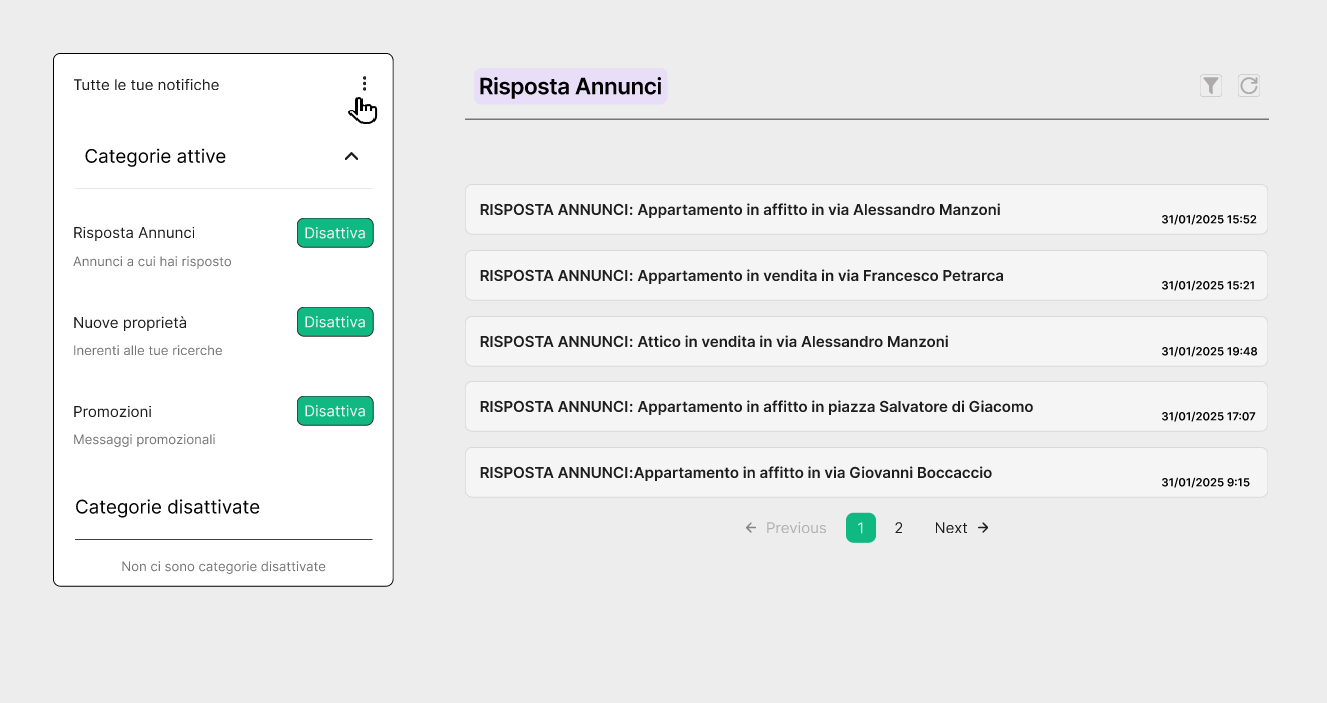
\includegraphics[width=0.7\textwidth]{Immagini/Mockup/notifiche/scenario principale/Pagina Lista Notifiche.png}\\
                Cockburn: step 1/2/3
            \end{tabular}
        };
        
        % Nodo per immagine 2 con didascalia sotto, posizionato a destra di img1
        \node (img2) [below=of img1] {
            \begin{tabular}{c}
                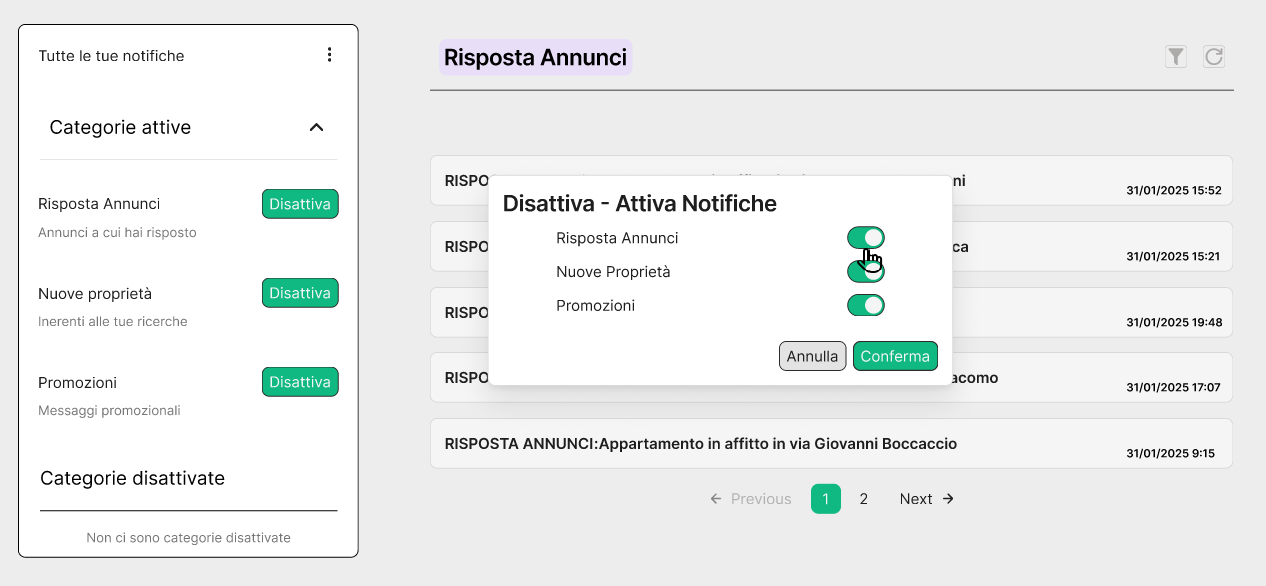
\includegraphics[width=0.7\textwidth]{Immagini/Mockup/notifiche/scenario principale/perDisattivareRisposte.png} \\
                Cockburn: step 4
            \end{tabular}
        };
        
        % Nodo per immagine 3 con didascalia sotto, posizionato sotto img2
        \node (img3) [below=of img2] {
            \begin{tabular}{c}
                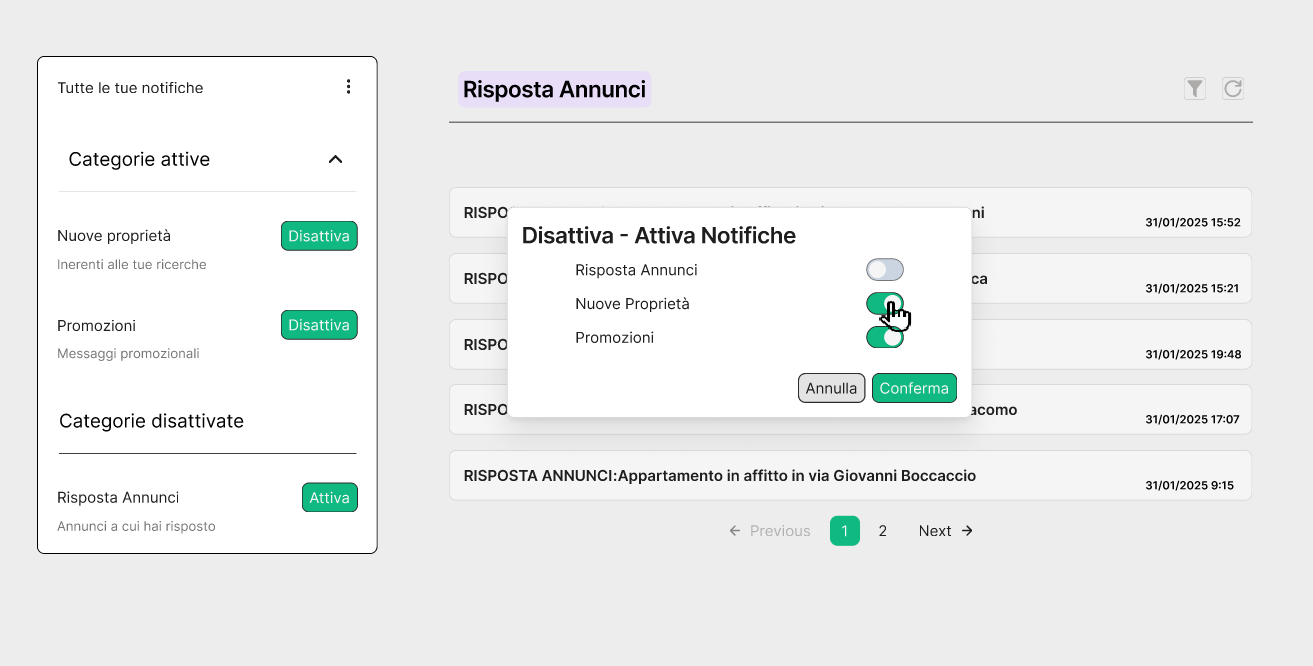
\includegraphics[width=0.7\textwidth]{Immagini/Mockup/notifiche/scenario principale/perDisattivareNueve.png} \\
                Cockburn: step 4
            \end{tabular}
        };

        
        % Disegna le frecce
        \draw[->, thick] (img1) -- (img2);
        \draw[->, thick] (img2) -- (img3);
        
    \end{tikzpicture}
    \caption{Mockup: scenario principale della tabella di Cockburn del caso d'uso disattiva/attiva categoria notifica}
    \label{fig:mockup_scenario_principale_parte1_disattiva_notifiche}
\end{figure}

\clearpage
\newpage

\begin{figure}[ht]
    \centering
    \begin{tikzpicture}[node distance=1.5cm and 1cm, auto]
      

         \node (img4){
            \begin{tabular}{c}
                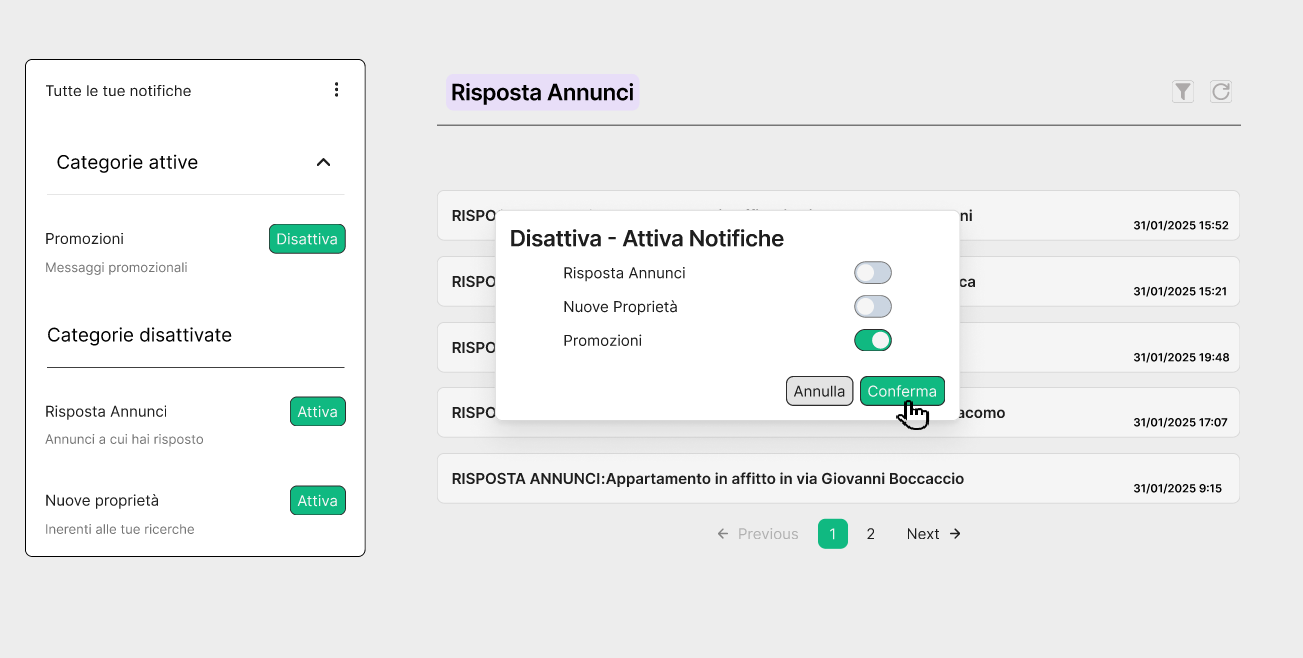
\includegraphics[width=0.7\textwidth]{Immagini/Mockup/notifiche/scenario principale/clickConferma.png} \\
                Cockburn: step 5
            \end{tabular}
        };

        \node (img5) [below=of img4] {
            \begin{tabular}{c}
                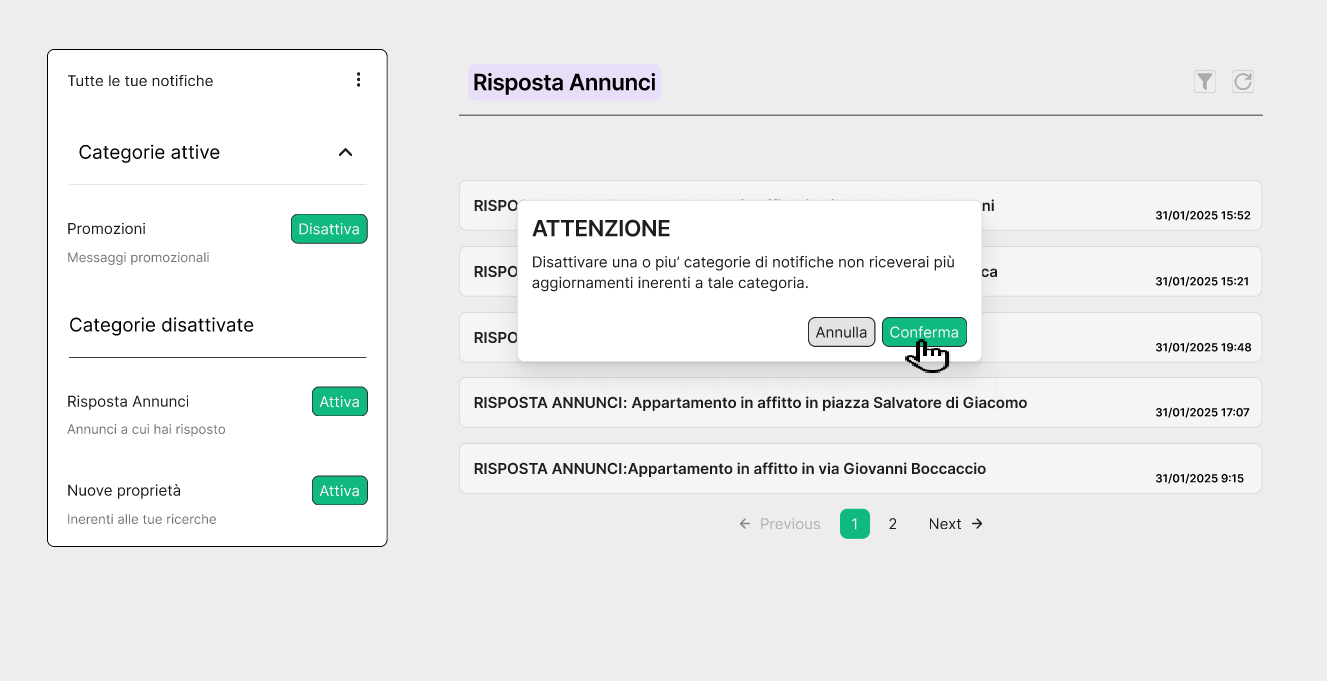
\includegraphics[width=0.7\textwidth]{Immagini/Mockup/notifiche/scenario principale/allerAvvisoDisattivazione.png} \\
                Cockburn: step 6/7
            \end{tabular}
        };

        \node (img6) [below=of img5] {
            \begin{tabular}{c}
                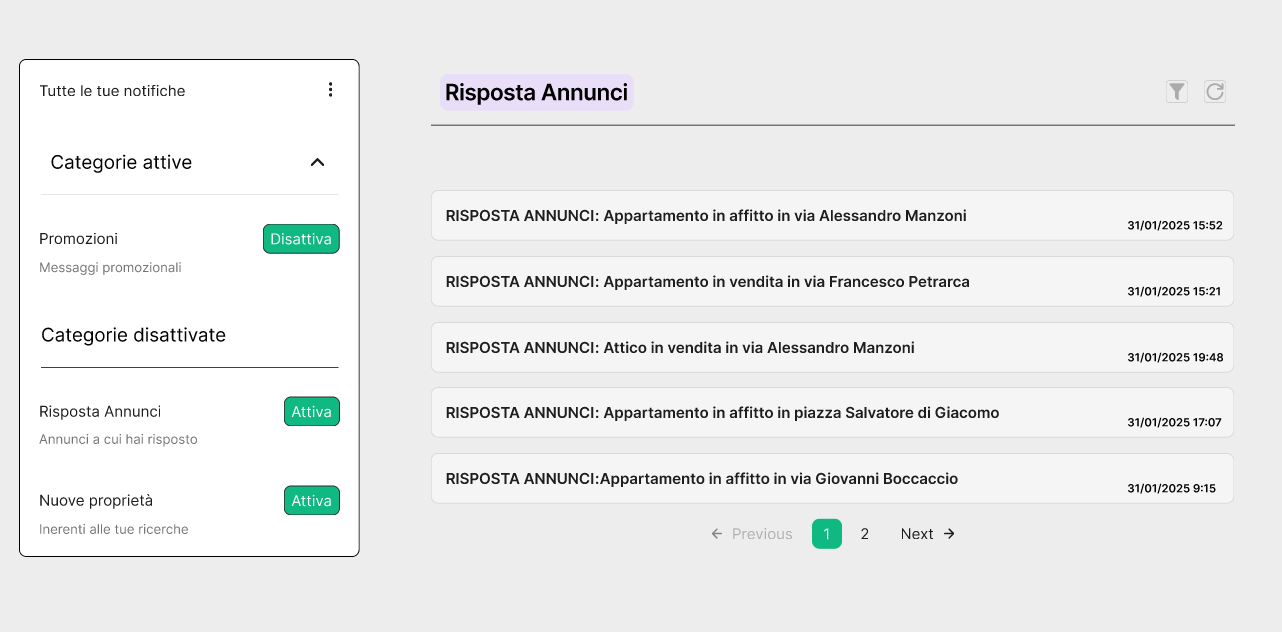
\includegraphics[width=0.7\textwidth]{Immagini/Mockup/notifiche/scenario principale/ScenarioPrincipaleCompletato.png} \\
                Conckburn: step 8/9/10
            \end{tabular}
        };
        
        % Disegna le frecce
        \draw[->, thick] (img4) -- (img5);
        \draw[->, thick] (img5) -- (img6);
        
    \end{tikzpicture}
    \caption{Parte 2 mockup: scenario principale della tabella di Cockburn del caso d'uso disattiva/attiva categoria notifica}
    \label{fig:mockup_scenario_principale_parte2_disattiva_notifiche}
\end{figure}

\clearpage
\newpage

\subsubsection{Estensione A: Disattivazione Notifiche dalla Visualizzazione di una Notifica}

Per offrire un maggiore controllo sulla gestione delle notifiche senza interrompere l’esperienza utente, il sistema permette di disattivare una categoria direttamente dalla visualizzazione di una notifica specifica. Questa variante è progettata per garantire una modifica consapevole delle preferenze, evitando azioni impulsive che potrebbero compromettere la ricezione di informazioni rilevanti.

\vspace{0.5cm}
\subsubsection{Interfaccia e Comportamento del Bottone}
Alla fine del testo di ogni notifica, se la relativa categoria è attiva, è presente un pulsante neutro con la dicitura “Disattiva notifiche”. Accanto al pulsante, un testo in grigio informa l’utente della funzione del pulsante, evitando ambiguità. L’utilizzo di colori non accesi e di un design discreto segue il principio della \textbf{gerarchia visiva} \cite{pieters2004}, scoraggiando azioni impulsive che potrebbero portare alla perdita involontaria di notifiche future.

\vspace{0.5cm}
\subsubsection{Modifica dello Stato e Feedback Visivo}
Quando l’utente clicca sul pulsante, il testo del pulsante cambia colore, diventando rosso, e il messaggio a fianco si aggiorna per sottolineare che la categoria di notifiche è stata disattivata. Questo utilizza il principio della \textbf{salienza visiva} \cite{nielsen1995}, enfatizzando il cambiamento e rendendo immediatamente chiara la conseguenza dell’azione.

\vspace{0.5cm}
\subsubsection{Incentivo alla Riattivazione}
Una volta disattivata una categoria tramite questa modalità, viene visualizzato un secondo pulsante con una call-to-action mirata per incentivare la riattivazione delle notifiche. Il design e il posizionamento del pulsante sfruttano il \textbf{principio dell’affordance} \cite{norman1988}, rendendo chiaro che l’utente ha la possibilità di tornare indietro sulla sua decisione in modo semplice e immediato.
\newline
Questa estensione si integra perfettamente con il modello generale di gestione delle notifiche, garantendo un’interazione fluida e coerente con le esigenze dell’utente. Nel caso in cui l’utente scelga di riattivare la categoria delle notifiche direttamente da una notifica, si passa all’\textbf{Estensione F}, che approfondisce questa modalità di gestione a partire dalle notifiche disattivate.
\begin{figure}[ht]
    \centering
    \begin{tikzpicture}[node distance=1.5cm and 1cm, auto]
        % Nodo per immagine 1 con didascalia sotto
        \node (img1) {
            \begin{tabular}{c}
                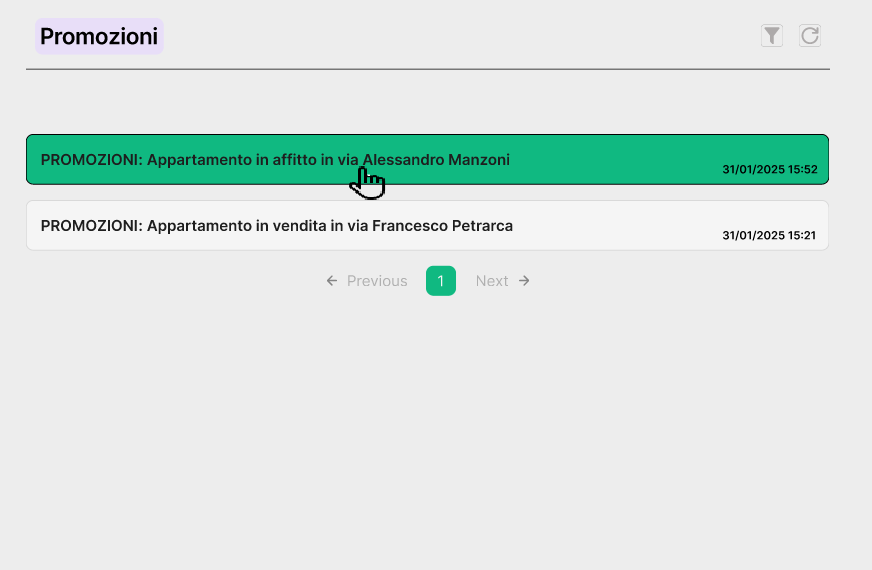
\includegraphics[width=0.4\textwidth]{Immagini/Mockup/notifiche/estensione A/clickNotifica.png} \\
                Cockburn: Extension A.2/A.3
            \end{tabular}
        };
        
        % Nodo per immagine 2 con didascalia sotto, posizionato a destra di img1
        \node (img2) [below=of img1] {
            \begin{tabular}{c}
                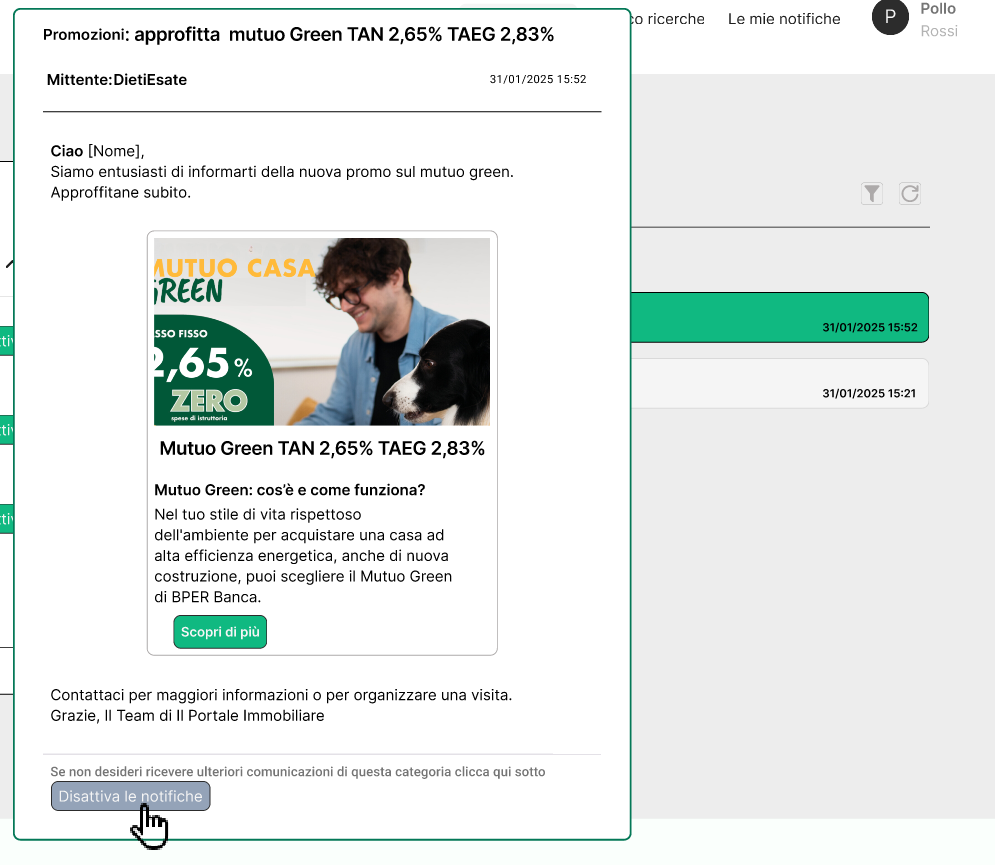
\includegraphics[width=0.4\textwidth]{Immagini/Mockup/notifiche/estensione A/clickDisattiva.png} \\
                Cockburn: Extension A.4
            \end{tabular}
        };
        
        % Nodo per immagine 3 con didascalia sotto, posizionato sotto img2
        \node (img3) [below=of img2] {
            \begin{tabular}{c}
                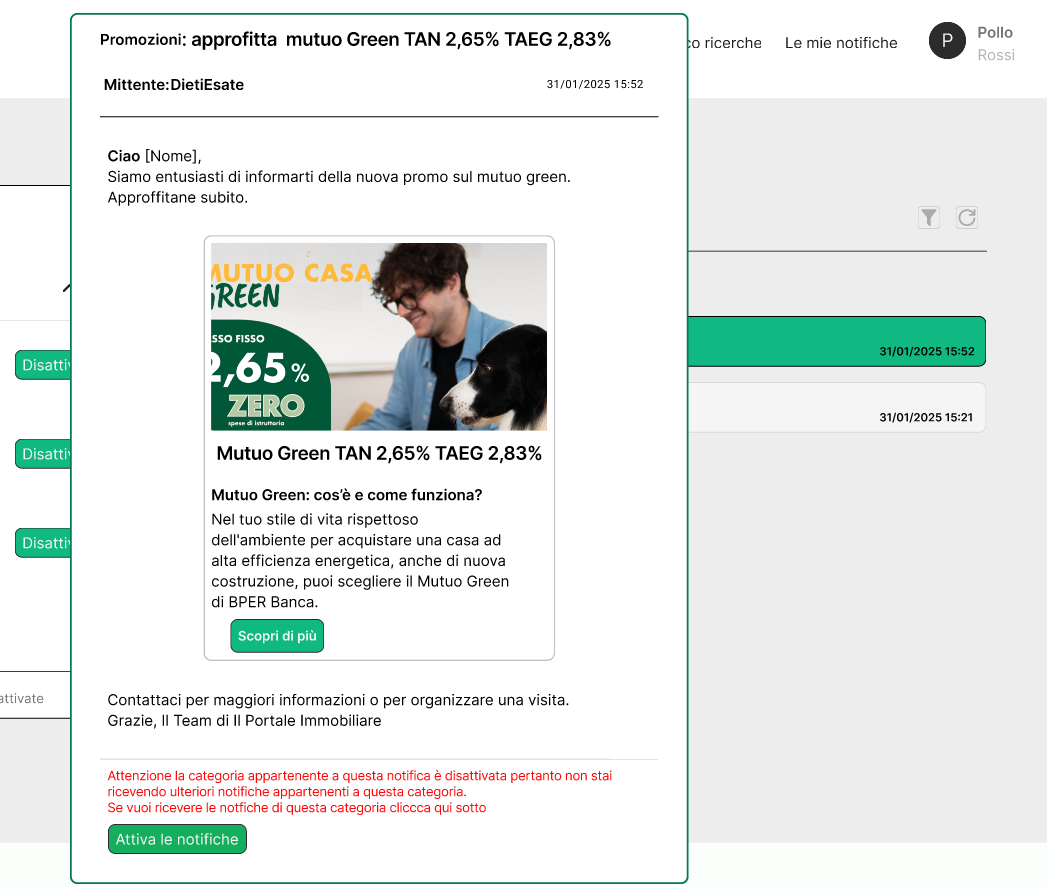
\includegraphics[width=0.4\textwidth]{Immagini/Mockup/notifiche/estensione A/disattivato.png} \\
                Cockburn: extension A.5
            \end{tabular}
        };
        
        % Disegna le frecce
        \draw[->, thick] (img1) -- (img2);
        \draw[->, thick] (img2) -- (img3);
      
    \end{tikzpicture}
    \caption{Mockup: estensione A della tabella di Cockburn del caso d'uso disattiva/attiva categoria notifica}
    \label{fig:mockup_estensione_A_disattiva_notifiche}
\end{figure}

\newpage


\clearpage
\newpage
\subsubsection{Estensione B: Ripristino di un Annuncio Precedente}
Se l’utente sceglie di \textbf{ripristinare l’annuncio precedente}, il sistema avvia un processo di caricamento per fornire un feedback visivo sulla ripresa dei dati. Sebbene i dati siano salvati localmente e il recupero sia immediato, un \textbf{indicatore di caricamento fittizio} viene mostrato per alcuni secondi prima di caricare la schermata.

Questa soluzione è basata sul principio della \textbf{coerenza con le aspettative dell’utente} \cite{shneiderman2004}. In un contesto digitale, un ripristino istantaneo potrebbe apparire innaturale e creare confusione. L’indicatore di caricamento:
\begin{itemize}
    \item Rafforza la percezione di un processo in corso, migliorando la trasparenza dell’operazione.
    \item Evita che l’utente si domandi se il recupero sia realmente avvenuto o se ci siano stati problemi tecnici.
    \item Contribuisce a una transizione più fluida tra stati dell’interfaccia.
\end{itemize}

Una volta completato il caricamento, il sistema presenta l’interfaccia con i dati precedentemente salvati, consentendo all’utente di riprendere il processo da dove era stato interrotto.


\begin{figure}[ht]
    \centering
    \begin{tikzpicture}[node distance=1.5cm and 1cm, auto]
        % Nodo per immagine 1 con didascalia sotto
        \node (img1) {
            \begin{tabular}{c}
                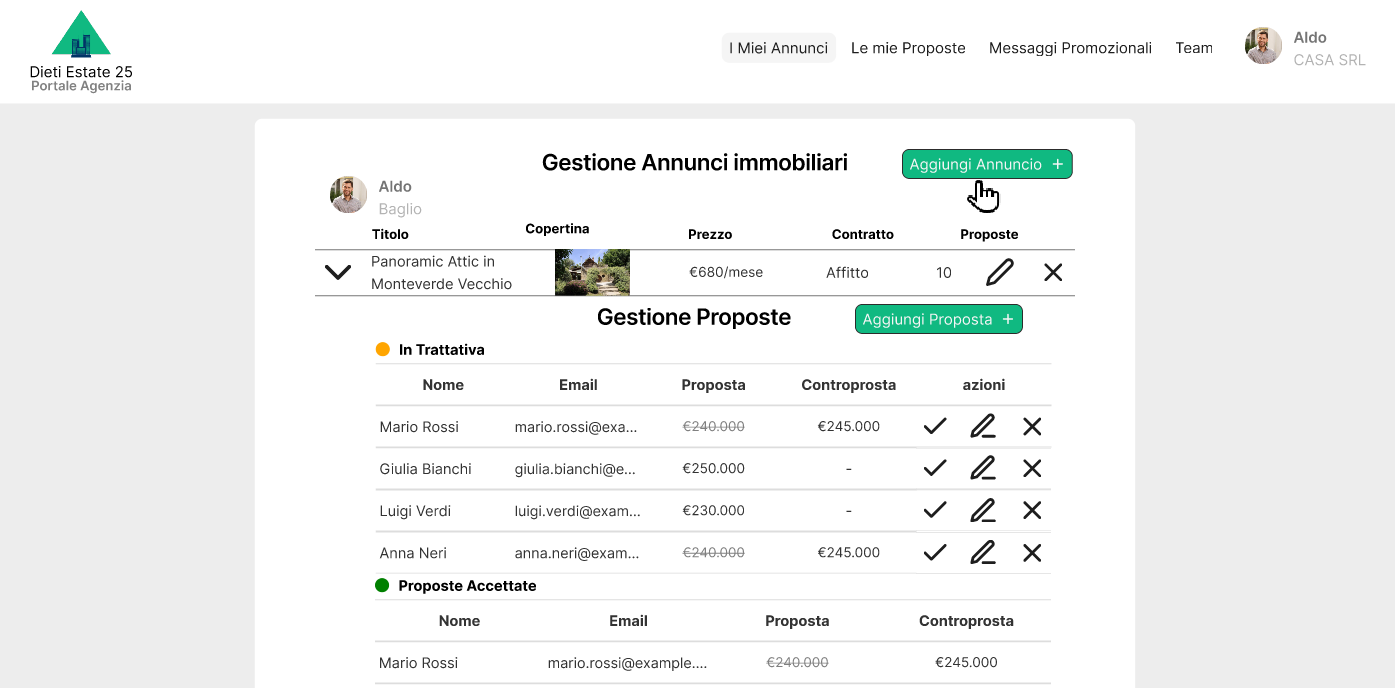
\includegraphics[width=0.7\textwidth]{Immagini/Mockup/aggiungi annuncio/estensione B/step1.png} \\
                click nuovo annuncio
            \end{tabular}
        };
        
        % Nodo per immagine 2 con didascalia sotto, posizionato a destra di img1
        \node (img2) [below=of img1] {
            \begin{tabular}{c}
                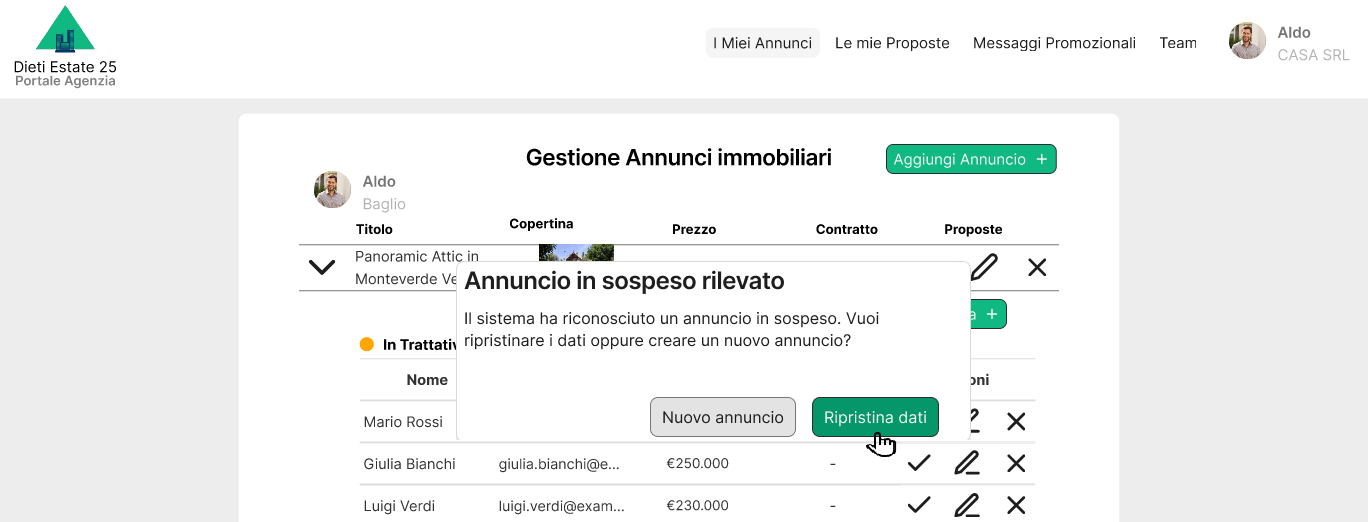
\includegraphics[width=0.7\textwidth]{Immagini/Mockup/aggiungi annuncio/estensione B/step2.png} \\
                Cockburn: extension B.2/B.3/B.4
            \end{tabular}
        };
        
        % Nodo per immagine 3 con didascalia sotto, posizionato sotto img2
        \node (img3) [below=of img2] {
            \begin{tabular}{c}
                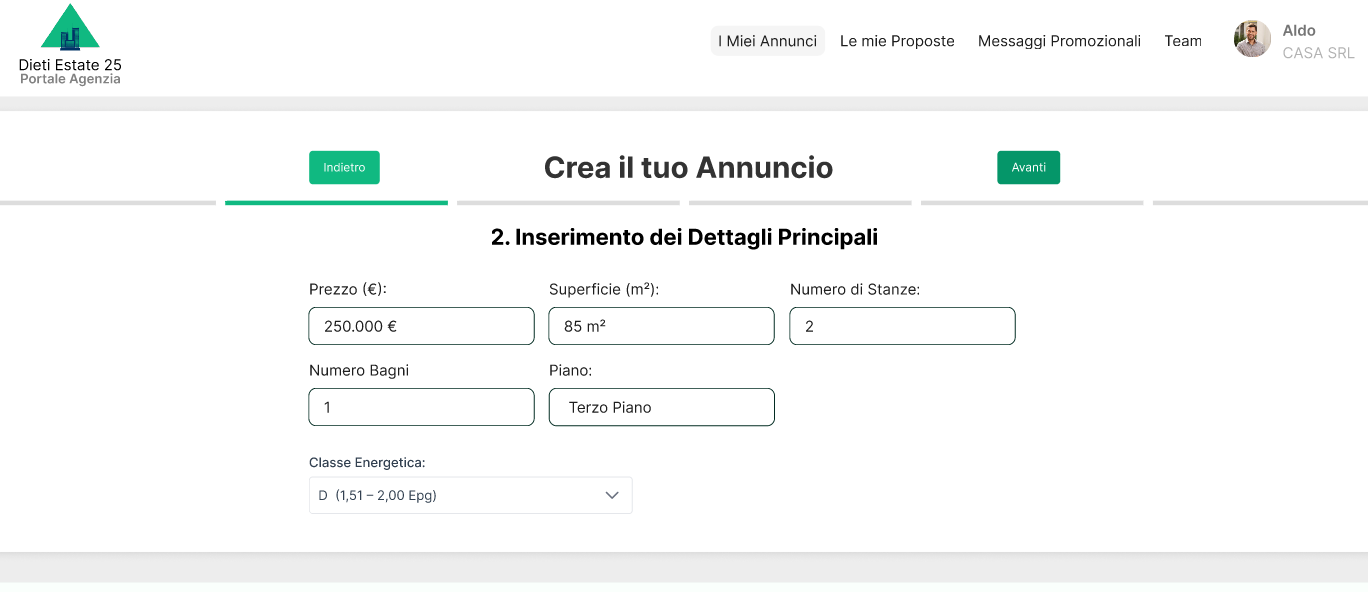
\includegraphics[width=0.7\textwidth]{Immagini/Mockup/aggiungi annuncio/estensione B/step3.png} \\
                Cockburn: extension B.5
            \end{tabular}
        };
        
        % Disegna le frecce
        \draw[->, thick] (img1) -- (img2);
        \draw[->, thick] (img2) -- (img3);
      
    \end{tikzpicture}
    \caption{Mockup: estensione B della tabella di Cockburn del caso d'uso nuovo annuncio}
    \label{fig:mockup_estensione_B_aggiungi_annuncio}
\end{figure}

\newpage



\input{Requisiti Del Software/Analisi dei Requisiti/Mockup/disattivazione notifiche/estensione c}

\clearpage
\newpage

\subsubsection{Estensione D: Modifica Rapida dello Stato delle Notifiche con Attivazione Immediata}

Questa variante rappresenta l’approccio duale dell’\textbf{Estensione C}, semplificando ulteriormente l’attivazione delle notifiche. L’obiettivo è ridurre i passaggi necessari per riattivare una categoria disattivata, mantenendo comunque un controllo chiaro sulla disattivazione.

\vspace{0.5cm}
\subsubsection{Interfaccia e Interazione}
Analogamente all’\textbf{Estensione C}, ogni categoria nella barra laterale dispone di un pulsante contestuale per modificarne lo stato. Il pulsante può assumere due stati:

\begin{itemize}
    \item \textbf{Attiva}, se la categoria è attualmente disabilitata.
    \item \textbf{Disattiva}, se la categoria è attualmente abilitata.
\end{itemize}

Le interazioni dell’utente variano a seconda dell’azione eseguita:

\begin{itemize}
    \item \textbf{Disattivazione di una categoria}:
    \begin{itemize}
        \item Al clic su \textbf{Disattiva}, appare un popup di conferma che informa l’utente sulle conseguenze della scelta, prevenendo azioni accidentali in linea con i principi di Nielsen \cite{nielsen1995}.
        \item Se confermata, la categoria viene spostata nella sezione delle notifiche disattivate tramite un’animazione di transizione.
        \item Il pulsante cambia stato, diventando \textbf{Attiva}, fornendo un feedback visivo chiaro sulla modifica.
    \end{itemize}
    
    \item \textbf{Attivazione di una categoria}:
    \begin{itemize}
        \item Al clic su \textbf{Attiva}, il sistema aggiorna immediatamente lo stato della notifica senza richiedere una conferma esplicita.
        \item La categoria viene spostata nella sezione delle notifiche attive con un’animazione fluida, applicando il principio della \textbf{gestalt della continuità} \cite{miller1956}.
        \item Il pulsante cambia stato in \textbf{Disattiva}, rendendo la modifica evidente e intuitiva.
    \end{itemize}
\end{itemize}

\subsubsection{Feedback Visivo e UX Design}
L’esperienza utente è ottimizzata tramite tecniche di design che garantiscono chiarezza e immediatezza:

\begin{itemize}
    \item \textbf{Popup di conferma per la disattivazione}: aiuta a prevenire errori e rende consapevole l’utente delle conseguenze della scelta \cite{nielsen1995}.
    \item \textbf{Animazione di transizione}: assicura una continuità visiva fluida nello spostamento delle categorie, migliorando la percezione del cambiamento \cite{miller1956}.
    \item \textbf{Aggiornamento immediato dello stato del pulsante}: il cambio di testo e colore riflette lo stato corrente della categoria, riducendo l’ambiguità e migliorando la prevedibilità dell’interazione.
\end{itemize}

Questa estensione semplifica l’attivazione delle notifiche, eliminando il passaggio della conferma e migliorando la fluidità dell’interazione, senza compromettere il controllo dell’utente sulla gestione delle proprie preferenze.

\begin{figure}[ht]
    \centering
    \begin{tikzpicture}[node distance=1.5cm and 1cm, auto]
        % Nodo per immagine 1 con didascalia sotto
        \node (img1) {
            \begin{tabular}{c}
                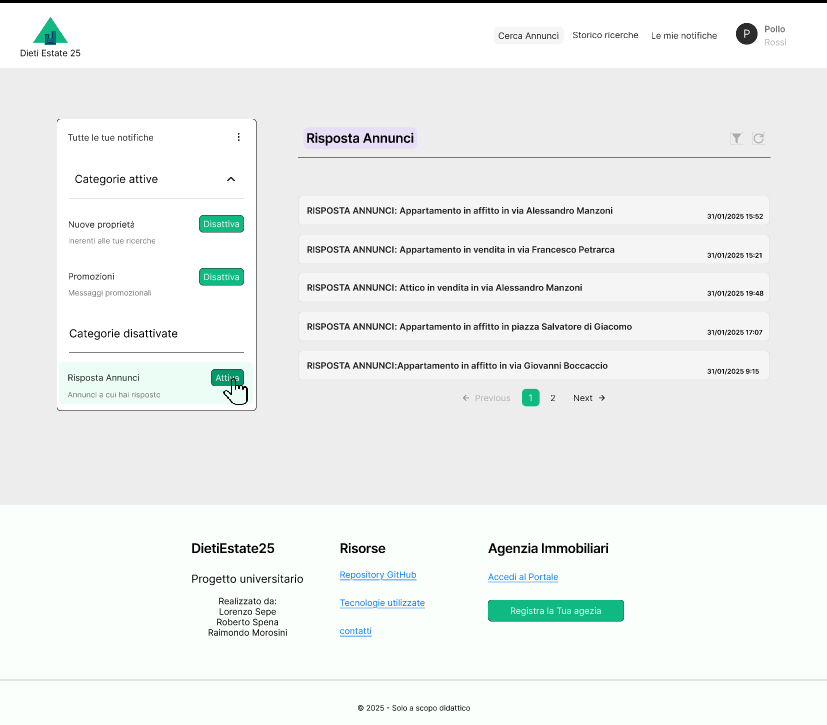
\includegraphics[width=0.6\textwidth]{Immagini/Mockup/notifiche/estensione D/clickAttiva.png} \\
                Cockburn: Extension D.2
            \end{tabular}
        };
        
        % Nodo per immagine 2 con didascalia sotto, posizionato a destra di img1
        \node (img2) [below=of img1] {
            \begin{tabular}{c}
                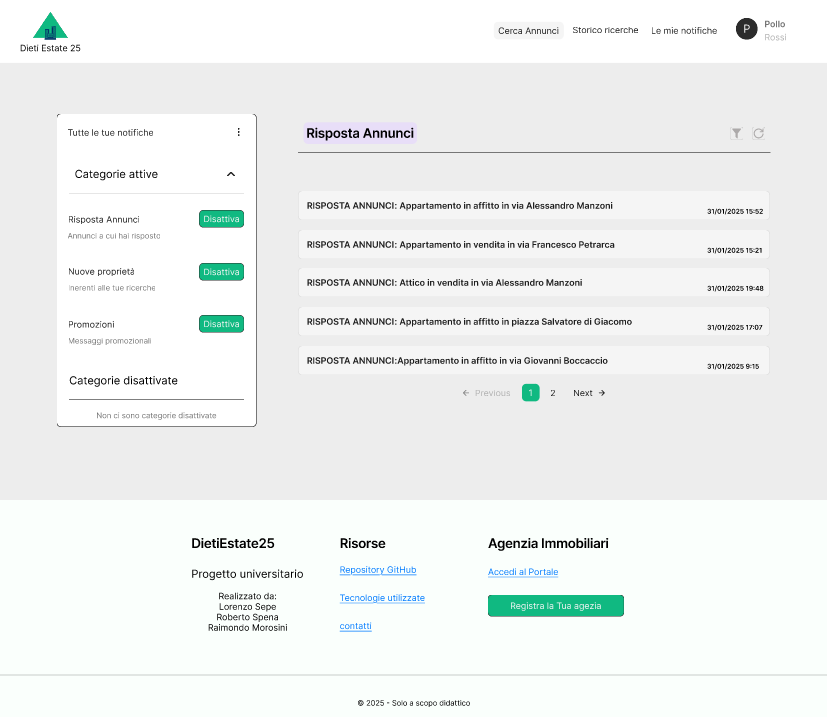
\includegraphics[width=0.6\textwidth]{Immagini/Mockup/notifiche/estensione D/attivato.png} \\
                Cockburn: step 8/9/10
            \end{tabular}
        };
        
        % Disegna le frecce
        \draw[->, thick] (img1) -- (img2);
      
    \end{tikzpicture}
    \caption{Mockup: estensione D della tabella di Cockburn del caso d'uso disattiva/attiva categoria notifica}
    \label{fig:mockup_estensione_D_disattiva_notifiche}
\end{figure}

\newpage



\clearpage
\newpage

\subsubsection{Estensione E: Errore Durante la Modifica dello Stato delle Categorie di Notifica}

Nel caso in cui si verifichi un errore durante il tentativo di modifica dello stato di una categoria di notifica, viene visualizzato un messaggio di errore sotto forma di un popup informativo. Il messaggio informa l'utente che la modifica non è riuscita e lo invita a riprovare più tardi, senza salvare le modifiche effettuate.

\vspace{0.5cm}
\subsubsection{Gestione dell'Errore e Feedback Utente} Il popup di errore presenta i seguenti elementi chiave: \begin{itemize} \item \textbf{Messaggio chiaro e informativo}: il messaggio comunica all'utente che l'operazione non è andata a buon fine, senza entrare in dettagli tecnici, per ridurre il rischio di frustrazione. L'utente viene anche informato che l'operazione non è stata completata e che le modifiche non sono state salvate. \item \textbf{Pulsante “Ok”}: consente all'utente di chiudere il popup e tornare all'interfaccia principale. Il pulsante di conferma è chiaro e consente di riprendere l'interazione senza indugi. \end{itemize}

\subsubsection{Principi di Design Applicati} L'approccio di gestione dell'errore in questa estensione si fonda sui seguenti principi di UX e usabilità: \begin{itemize} \item \textbf{Visibilità dello stato del sistema} \cite{nielsen1995}: l'errore è comunicato all'utente attraverso un popup che evidenzia chiaramente che il sistema non è riuscito a completare l'operazione. \item \textbf{Prevenzione degli errori} \cite{nielsen1995}: sebbene l'errore non possa essere evitato completamente, il sistema offre un feedback immediato e comprensibile, impedendo all'utente di rimanere confuso o incerto sullo stato dell'operazione. \item \textbf{Semplicità e chiarezza} \cite{nielsen1995}: il messaggio di errore è semplice e diretto, senza sovraccaricare l'utente con informazioni tecniche. L'invito a riprovare più tardi mantiene il flusso di lavoro semplice e lineare. \item \textbf{Controllo dell'utente} \cite{norman1988}: l'utente ha il pieno controllo sulla gestione dell'errore, poiché il popup permette di chiudere facilmente l'interfaccia e riprendere l'attività, mantenendo un'esperienza utente fluida. \end{itemize}

Questa soluzione di gestione dell'errore è progettata per garantire un'esperienza utente chiara e senza frustrazioni, minimizzando il disagio derivante da errori tecnici imprevisti e offrendo un percorso semplice per riprendere l'interazione.
\begin{figure}[ht]
    \centering
    \begin{tikzpicture}[node distance=1.5cm and 1cm, auto]
        % Nodo per immagine 1 con didascalia sotto
        \node (img1) {
            \begin{tabular}{c}
                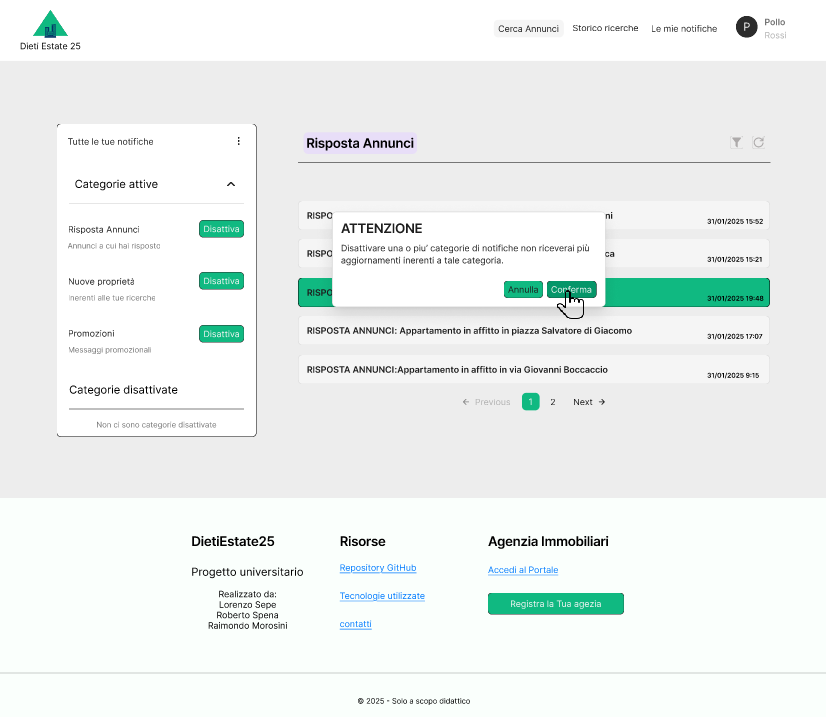
\includegraphics[width=0.6\textwidth]{Immagini/Mockup/notifiche/estensione E/click conferma.png} \\
                Cockburn: step 7
            \end{tabular}
        };
        
        % Nodo per immagine 2 con didascalia sotto, posizionato a destra di img1
        \node (img2) [below=of img1] {
            \begin{tabular}{c}
                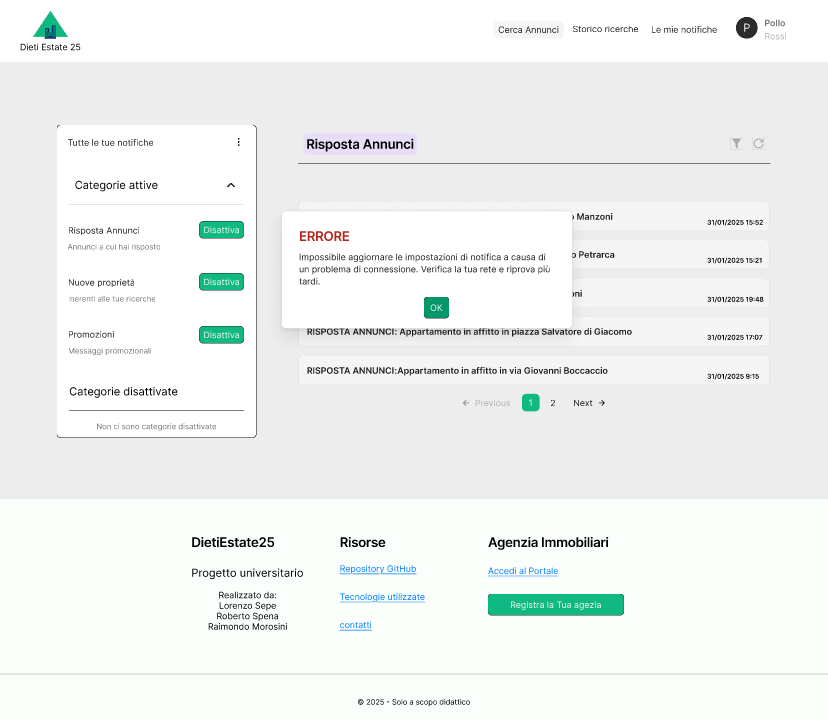
\includegraphics[width=0.6\textwidth]{Immagini/Mockup/notifiche/estensione E/errore.png} \\
                Cockburn: Extension E.7/E.8
            \end{tabular}
        };
        
        % Disegna le frecce
        \draw[->, thick] (img1) -- (img2);
      
    \end{tikzpicture}
    \caption{Mockup: estensione E della tabella di Cockburn del caso d'uso disattiva/attiva categoria notifica}
    \label{fig:tikz_flow}
\end{figure}

\newpage



\clearpage
\newpage

\subsubsection{Estensione F: Riattivazione Notifiche dalle Notifiche Disattivate}

Questa estensione consente all’utente di riattivare una categoria di notifiche direttamente da una notifica precedentemente ricevuta e appartenente a una categoria disattivata. L’obiettivo è fornire un meccanismo immediato per ripristinare le notifiche quando l’utente si rende conto della loro utilità.

\vspace{0.5cm}
\subsubsection{Indicazione dello Stato e Call-to-Action}
Quando una notifica proviene da una categoria disattivata, il sistema mostra un messaggio di avviso evidenziato che informa l’utente che non riceverà più aggiornamenti simili. Il pulsante associato cambia stato e diventa un invito all’azione con il testo “Riattiva notifiche”. Questo sfrutta il \textbf{principio della reversibilità} \cite{shneiderman2004}, permettendo all’utente di annullare la decisione precedente senza difficoltà.

\vspace{0.5cm}
\subsubsection{Feedback Visivo e Conferma della Riattivazione}
Alla pressione del pulsante, il testo cambia colore in verde e il messaggio informativo si aggiorna, confermando che le notifiche per quella categoria sono state riattivate. Il sistema può fornire un’ulteriore conferma con un breve messaggio di notifica o una vibrazione del dispositivo per enfatizzare l’azione completata.

\vspace{0.5cm}
\subsubsection{Coerenza con il Modello di Gestione Notifiche}
Questa estensione rafforza la coerenza dell’interfaccia di gestione delle notifiche, mantenendo le scelte dell’utente sempre modificabili e promuovendo un’interazione trasparente e prevedibile. L’utente può così gestire le notifiche senza dover accedere necessariamente alla schermata delle impostazioni, riducendo il carico cognitivo e migliorando l’usabilità complessiva del sistema.\begin{figure}[ht]
    \centering
    \begin{tikzpicture}[node distance=1.5cm and 1cm, auto]
        % Nodo per immagine 1 con didascalia sotto
        \node (img1) {
            \begin{tabular}{c}
                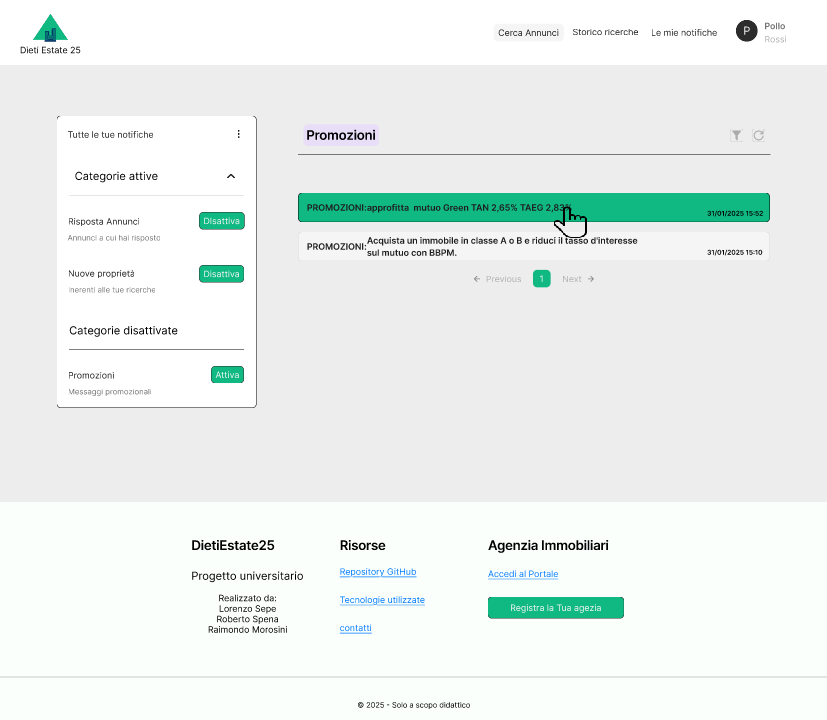
\includegraphics[width=0.4\textwidth]{Immagini/Mockup/notifiche/estensione F/clickNotifica.png} \\
                Cockburn: Extension F.2
            \end{tabular}
        };
        
        % Nodo per immagine 2 con didascalia sotto, posizionato a destra di img1
        \node (img2) [below=of img1] {
            \begin{tabular}{c}
                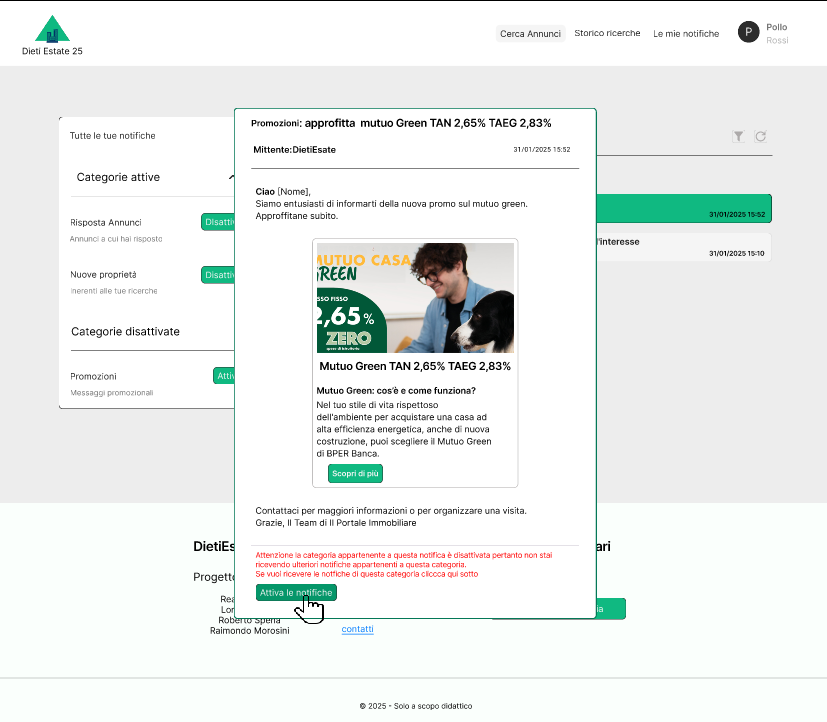
\includegraphics[width=0.4\textwidth]{Immagini/Mockup/notifiche/estensione F/clickAttiva.png} \\
                Cockburn: Extension F.3
            \end{tabular}
        };
        
        % Nodo per immagine 3 con didascalia sotto, posizionato sotto img2
        \node (img3) [below=of img2] {
            \begin{tabular}{c}
                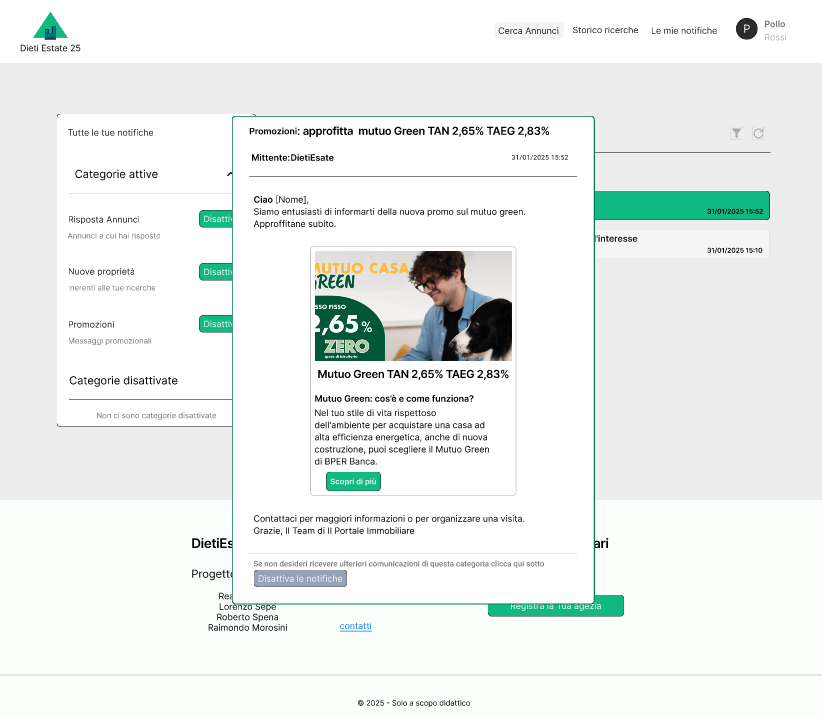
\includegraphics[width=0.4\textwidth]{Immagini/Mockup/notifiche/estensione F/attivato.png} \\
                Cockburn: Extension F.4/F.5
            \end{tabular}
        };
        
        % Disegna le frecce
        \draw[->, thick] (img1) -- (img2);
        \draw[->, thick] (img2) -- (img3);
      
    \end{tikzpicture}
    \caption{Mockup: estensione F della tabella di Cockburn del caso d'uso disattiva/attiva categoria notifica}
    \label{fig:mockup_estensione_F_disattiva_notifiche}
\end{figure}

\newpage




\subsection{Caso d'Uso: Controproposta di un'Offerta}

Il caso d’uso Controproposta di un’offerta è stato progettato seguendo la stessa logica di interazione non intrusiva adottata per altre operazioni simili.
L’obiettivo principale è mantenere la continuità del contesto visivo, riducendo al minimo le interruzioni nel flusso di lavoro dell’utente. Per questo motivo, l’azione viene gestita all’interno di una finestra modale (popup) che consente di operare senza abbandonare la vista principale.

\vspace{0.5cm}
\subsubsection{Struttura e Flusso dell’Interazione}
L’interazione si articola in più fasi distinte, ognuna delle quali mira a garantire chiarezza e controllo all’utente:
\begin{itemize}
	\item \textbf{Popup iniziale}: la finestra modale mostra i dettagli della proposta selezionata (mittente, testo sintetico e valore corrente) e include un campo dedicato all’inserimento del nuovo valore della controproposta.
	In calce è presente un pulsante di azione principale con etichetta \textbf{«Invia controproposta»}.
	
	\item \textbf{Conferma dell’invio}: al clic su \textbf{«Invia controproposta»}, viene visualizzato un dialog di conferma per prevenire invii accidentali.  
	I pulsanti di conferma e annullamento sono caratterizzati da colori neutri, così da differenziarli visivamente dalle azioni primarie della piattaforma e migliorare la leggibilità percettiva \cite{nielsen1995}.
	
	\item \textbf{Feedback di caricamento}: dopo la conferma, il sistema mostra una barra di avanzamento stilizzata con i colori istituzionali dell’applicazione.  
	Anche in presenza di tempi di risposta brevi, viene introdotto un lieve ritardo percettivo per garantire un feedback visivo chiaro sull’elaborazione in corso \cite{shneiderman2004}.
	
	
\end{itemize}

\vspace{0.5cm}
\subsubsection{Esito dell’Operazione e Aggiornamento della Lista}
Al completamento dell’operazione, il sistema applica una serie di aggiornamenti automatici per riflettere lo stato corrente:
\begin{itemize}
	\item la finestra modale viene chiusa automaticamente;
	\item nella lista delle proposte, la voce corrispondente viene aggiornata con il nuovo valore della controproposta;
	\item il testo della proposta precedente può essere troncato o sintetizzato per preservare la leggibilità complessiva della tabella;
	\item lo stato della proposta viene aggiornato a \emph{«Controproposta inviata»}, rendendo immediatamente visibile l’esito dell’azione.
\end{itemize}

\vspace{0.5cm}
\subsubsection{Considerazioni di Usabilità e Sicurezza}
La soluzione basata su finestra modale garantisce un’esperienza utente coerente con i principi di usabilità e sicurezza dell’interfaccia:
\begin{itemize}
	\item \textbf{Continuità contestuale}: l’utente rimane all’interno del proprio flusso operativo, con possibilità di annullamento rapido.
	\item \textbf{Prevenzione degli errori}: la doppia conferma riduce il rischio di invii accidentali, in linea con le \textbf{heuristiche di Nielsen} per la prevenzione degli errori \cite{nielsen1995}.
	\item \textbf{Feedback percettivo affidabile}: la barra di caricamento fornisce un riscontro visivo chiaro sullo stato del processo, migliorando la percezione di controllo dell’utente \cite{wickens2008}.
\end{itemize}

Dal punto di vista della gestione dei dati, è raccomandata la validazione \textit{server-side} del valore della controproposta e l’applicazione di politiche di accesso coerenti con i principi di \textbf{minimizzazione delle informazioni} e \textbf{sicurezza dei dati}.
In caso di errore di invio, il sistema deve presentare messaggi chiari e impedire l’invio ripetuto della stessa controproposta fino al completamento dell’elaborazione, prevenendo possibili condizioni di \textit{race} o incongruenze nei dati.

\begin{figure}[H]
	\centering
	\begin{tikzpicture}[node distance=1.5cm and 1cm, auto]
		% Nodo per immagine 1 con didascalia sotto
		\node (img1) {
			\begin{tabular}{c}
				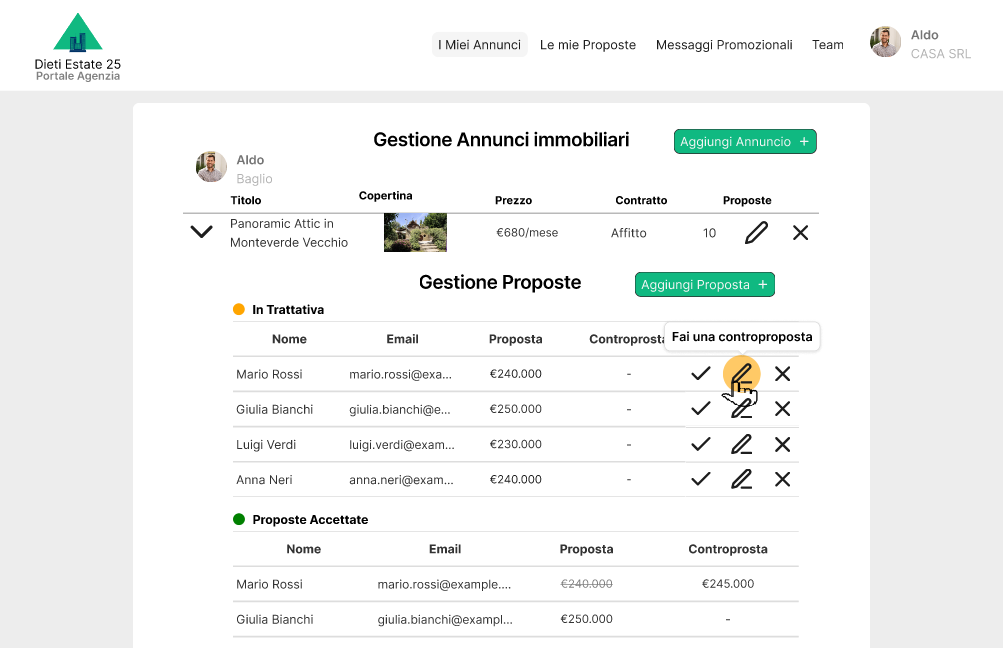
\includegraphics[width=0.7\textwidth]{Immagini/Mockup/controproposte/scenario principale/clickControproposta.png} \\
				Cockburn: step 1/2/3/4
			\end{tabular}
		};
		
		% Nodo per immagine 2 con didascalia sotto, posizionato a destra di img1
		\node (img2) [below=of img1] {
			\begin{tabular}{c}
				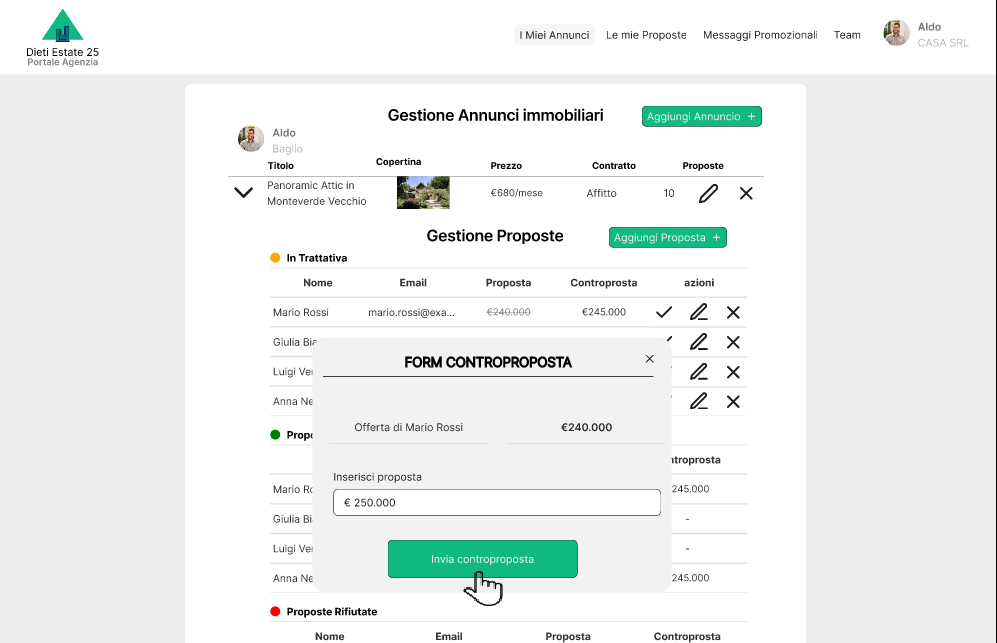
\includegraphics[width=0.7\textwidth]{Immagini/Mockup/controproposte/scenario principale/ClickInviaControproposta.png} \\
				Cockburn: step 5/6/7
			\end{tabular}
		};
		
		% Nodo per immagine 3 con didascalia sotto, posizionato sotto img2
		\node (img3) [below=of img2] {
			\begin{tabular}{c}
				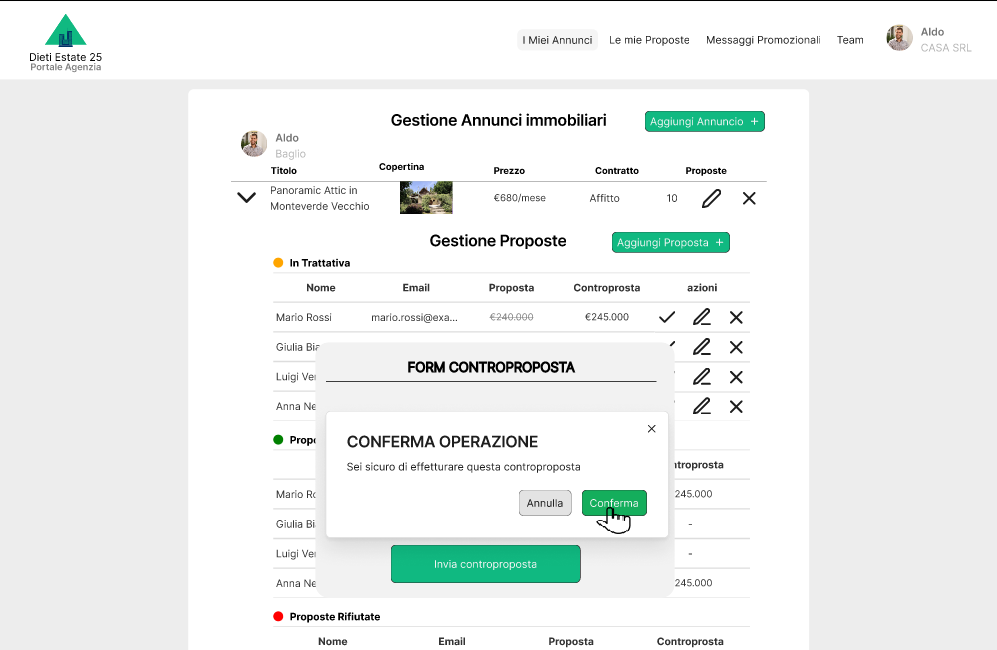
\includegraphics[width=0.7\textwidth]{Immagini/Mockup/controproposte/scenario principale/allertConfermaInvio.png} \\
				Cockburn: step 8/9/10
			\end{tabular}
		};
		
		% Disegna le frecce
		\draw[->, thick] (img1) -- (img2);
		\draw[->, thick] (img2) -- (img3);
		
	\end{tikzpicture}
	\caption{Mockup: scenario principale della tabella di Cockburn del caso d'uso: Fare una controproposta a un'offerta.}
	\label{fig:tikz_flow}
\end{figure}

\newpage

\begin{figure}[H]
	\centering
	\includegraphics[width=0.7\linewidth]{"Immagini/Mockup/controproposte/scenario principale/visualizzazioneControproposta"}
	\caption[Visualizzazione della controproposta]{}
	\label{fig:visualizzazionecontroproposta}
\end{figure}

\begin{figure}[H]
	\centering
	\begin{tikzpicture}[node distance=1.5cm and 1cm, auto]
		% Nodo per immagine 2 con didascalia sotto, posizionato a destra di img1
		\node (img1) {
			\begin{tabular}{c}
				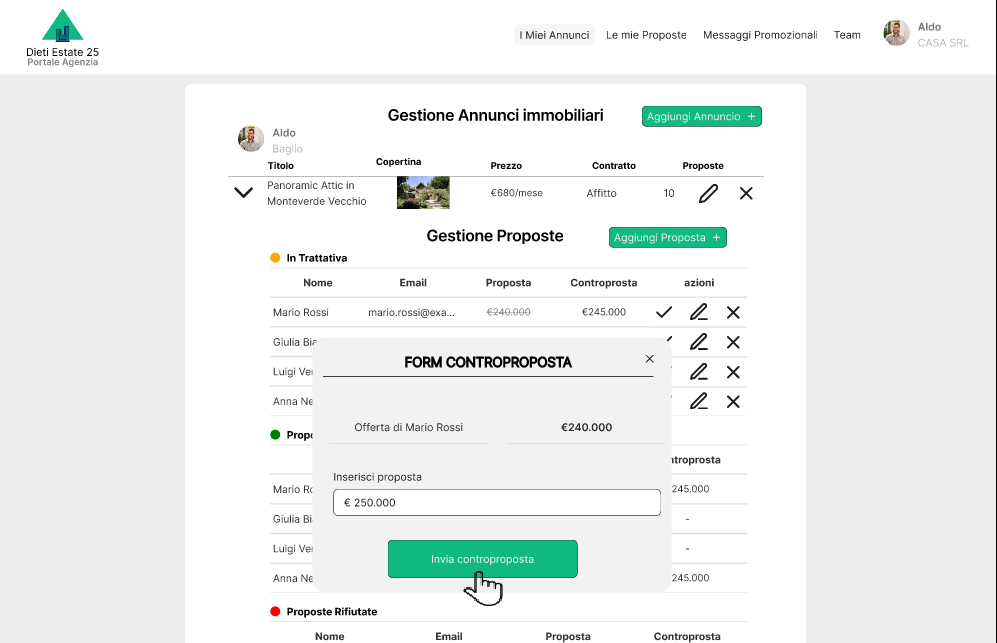
\includegraphics[width=0.7\textwidth]{Immagini/Mockup/controproposte/scenario principale/ClickInviaControproposta.png} \\
				Cockburn: step 6.A
			\end{tabular}
		};
		
		% Nodo per immagine 3 con didascalia sotto, posizionato sotto img2
		\node (img2) [below=of img1] {
			\begin{tabular}{c}
				\includegraphics[width=0.7\textwidth]{Immagini/Mockup/controproposte/Extensions A/MessaggioDiErrore.png} \\
				Cockburn: step 7.A
			\end{tabular}
		};
		
		% Disegna le frecce
		\draw[->, thick] (img1) -- (img2);
		
	\end{tikzpicture}
	\caption{Mockup: Extension A della tabella di Cockburn del caso d'uso: Fare una controproposta a un'offerta.}
	\label{fig:tikz_flow}
\end{figure}

\newpage




\newpage

\begin{figure}[H]
	\centering
	\begin{tikzpicture}[node distance=1.5cm and 1cm, auto]
		% Nodo per immagine 2 con didascalia sotto, posizionato a destra di img1
		\node (img1) {
			\begin{tabular}{c}
				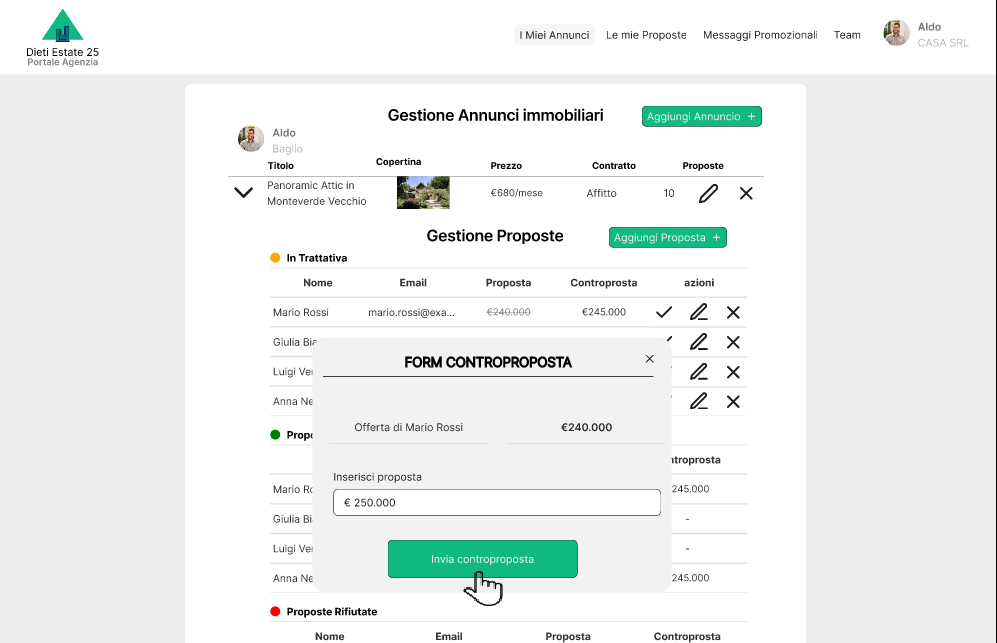
\includegraphics[width=0.7\textwidth]{Immagini/Mockup/controproposte/scenario principale/ClickInviaControproposta.png} \\
				Cockburn: step 7.B
			\end{tabular}
		};
		
		% Nodo per immagine 3 con didascalia sotto, posizionato sotto img2
		\node (img2) [below=of img1] {
			\begin{tabular}{c}
				\includegraphics[width=0.7\textwidth]{Immagini/Mockup/controproposte/Extensions B/MessaggioDiErrore.png} \\
				Cockburn: step 8.B
			\end{tabular}
		};
		
		% Disegna le frecce
		\draw[->, thick] (img1) -- (img2);
		
	\end{tikzpicture}
	\caption{Mockup: Extension B della tabella di Cockburn del caso d'uso: Fare una controproposta a un'offerta.}
	\label{fig:tikz_flow}
\end{figure}

\newpage




\newpage

subsubsection{Estensione C: Errore di Salvataggio della Controproposta}

In alcune circostanze, l’invio della controproposta può fallire a causa di problemi di connessione o di errori del server.  
Il sistema gestisce questa eventualità mostrando all’utente un chiaro feedback visivo sull’esito dell’operazione.

\subsubsection{Gestione dell’Errore e Comunicazione all’Utente}
Dopo aver cliccato su \textbf{“Invia controproposta”}, viene mostrato un breve stato di caricamento.  
Se il salvataggio non va a buon fine, compare un pop-up di allerta che informa l’agente dell’errore e della mancata registrazione della controproposta.

L’utente può chiudere l’allerta e tentare nuovamente l’operazione una volta ristabilita la connessione.  
Questo comportamento supporta la \textbf{recuperabilità dall’errore}, assicurando che l’utente non perda il lavoro svolto e possa riprovare senza dover reinserire tutti i dati.

\begin{figure}[H]
	\centering
	\begin{tikzpicture}[node distance=1.5cm and 1cm, auto]
		% Nodo per immagine 2 con didascalia sotto, posizionato a destra di img1
		\node (img1) {
			\begin{tabular}{c}
				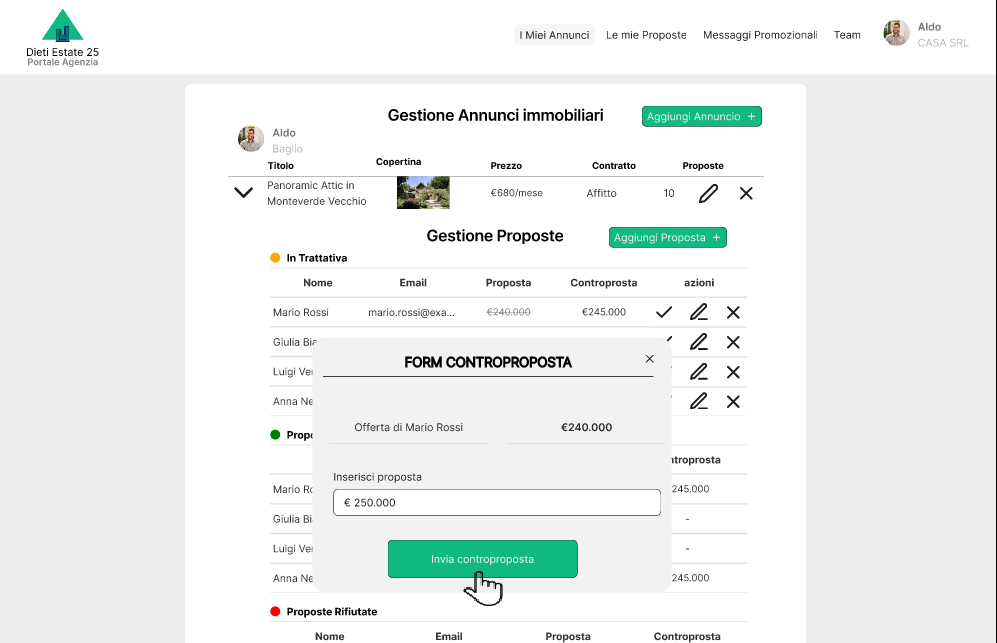
\includegraphics[width=0.7\textwidth]{Immagini/Mockup/controproposte/scenario principale/ClickInviaControproposta.png} \\
				Cockburn: step 7.C/8.C
			\end{tabular}
		};
		
		% Nodo per immagine 3 con didascalia sotto, posizionato sotto img2
		\node (img2) [below=of img1] {
			\begin{tabular}{c}
				\includegraphics[width=0.7\textwidth]{Immagini/Mockup/controproposte/Extensions C/MessaggioDiErrore.png} \\
				Cockburn: step 9.C
			\end{tabular}
		};
		
		% Disegna le frecce
		\draw[->, thick] (img1) -- (img2);
		
	\end{tikzpicture}
	\caption{Mockup: Extension C della tabella di Cockburn del caso d'uso: Fare una controproposta a un'offerta.}
	\label{fig:tikz_flow}
\end{figure}

\newpage




\subsubsection{Estensione D: Annullamento della Controproposta nella Finestra di Conferma}

Nel caso in cui, all’interno della finestra di conferma, l’agente scelga di annullare l’invio della controproposta, il sistema non procede con il salvataggio dei dati né con l’invio della notifica all’utente.

\subsubsection{Comportamento del Sistema}
Se l’agente clicca su \textbf{“Annulla”} invece di confermare l’operazione, la finestra di dialogo viene chiusa e il flusso ritorna al punto 6 dello scenario principale, consentendo la modifica o la revisione del prezzo proposto.  

Questa interazione segue il principio del \textbf{controllo da parte dell’utente} \cite{nielsen1995}, garantendo la possibilità di interrompere o modificare l’azione prima della sua esecuzione definitiva.
\begin{figure}[H]
	\centering
	\begin{tikzpicture}[node distance=1.5cm and 1cm, auto]
		% Nodo per la finestra di conferma
		\node (img1) {
			\begin{tabular}{c}
				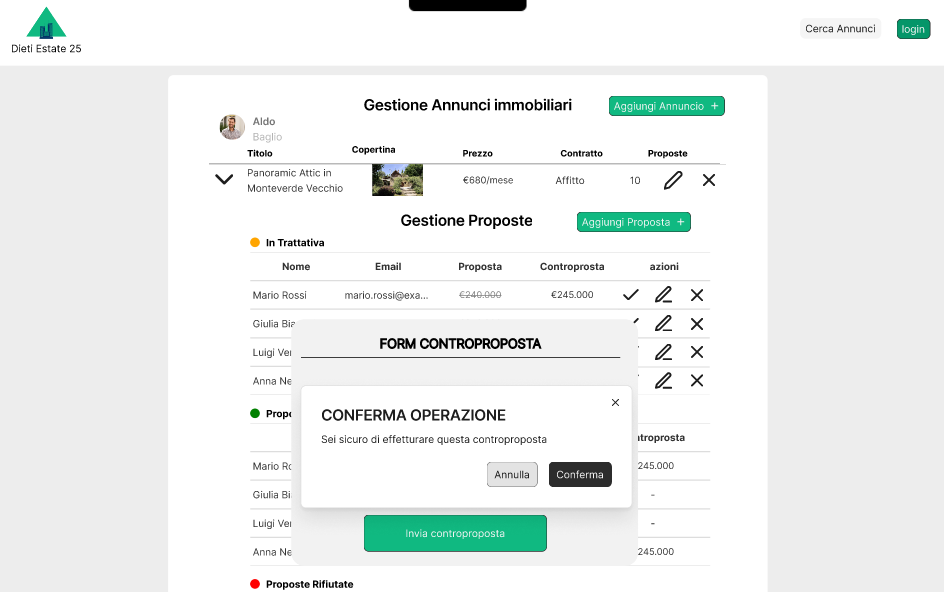
\includegraphics[width=0.7\textwidth]{Immagini/Mockup/controproposte/Extensions D/FinestraConfermaControproposta.png} \\
				Cockburn: step 9.D
			\end{tabular}
		};

		% Nodo per l'azione di annullamento e ritorno alla schermata di modifica
		\node (img2) [below=of img1] {
			\begin{tabular}{c}
				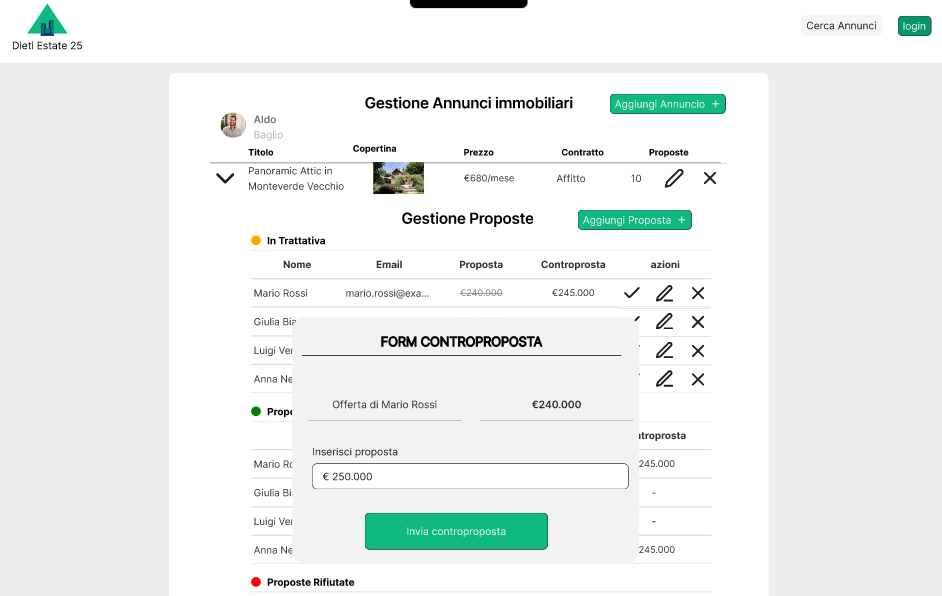
\includegraphics[width=0.7\textwidth]{Immagini/Mockup/controproposte/Extensions D/SchermataContropropostaAnnullata.png} \\
				Cockburn: ritorno al punto 6
			\end{tabular}
		};

		% Disegna la freccia tra i due step
		\draw[->, thick] (img1) -- (img2);

	\end{tikzpicture}
	\caption{Mockup: Extension D della tabella di Cockburn del caso d'uso: Fare una controproposta a un'offerta.}
	\label{fig:tikz_flow_extensionD}
\end{figure}

\newpage




\clearpage
\newpage



\subsection{Caso d'Uso: Registrazione di un Nuovo Agente}

Il caso d’uso «Registra nuovo agente» è stato progettato con l’obiettivo di garantire un’esperienza utente fluida e coerente con il resto dell’interfaccia, evitando interruzioni del contesto visivo. Per questo motivo, si è scelto di non introdurre una schermata dedicata, ma di utilizzare una finestra modale (popup), che consente all’utente di eseguire l’operazione senza abbandonare la vista corrente.

\vspace{0.5cm}
\subsubsection{Struttura e Flusso dell’Interazione}
L’interazione si articola in più fasi, guidando l’utente in modo progressivo e controllato:
\begin{itemize}
	\item \textbf{Popup iniziale}: contiene un form per l’inserimento dei dati anagrafici e professionali dell’agente, accompagnato da un unico pulsante in calce con etichetta «Registra nuovo utente».
	\item \textbf{Conferma dell’operazione}: al clic sul pulsante, viene mostrato un \textit{dialog} di doppia conferma per ridurre il rischio di azioni involontarie. I pulsanti di conferma e annullamento sono caratterizzati da colori neutri, in modo da distinguerli visivamente dall’azione primaria dell’applicazione.
	\item \textbf{Feedback di caricamento}: dopo la conferma, il sistema mostra una barra di avanzamento stilizzata con i colori istituzionali del sito. Anche nei casi in cui l’operazione risulti immediata, la barra può essere mantenuta visibile per una breve durata, al fine di fornire un riscontro percettivo chiaro e rassicurante \cite{nielsen1995}.
\end{itemize}

\vspace{0.5cm}
\subsubsection{Messaggio di Conferma e Gestione delle Credenziali}
Al completamento del processo di registrazione, il sistema visualizza un messaggio di successo che informa l’utente dell’avvenuta generazione delle credenziali di accesso.
Il pulsante contestuale assume l’etichetta \textbf{«Copia credenziali»}, permettendo di salvare in modo sicuro i dati generati.
Per prevenire la perdita delle credenziali, la chiusura del dialog è temporaneamente disabilitata fino a quando l’utente non conferma l’avvenuta copia.

\vspace{0.5cm}
\subsubsection{Visualizzazione e Sicurezza dei Dati}
In linea con i principi di \textbf{minimizzazione dei dati} e \textbf{sicurezza dell’informazione} \cite{wickens2008}, la visualizzazione completa delle credenziali non è obbligatoria:
il sistema privilegia la protezione dei dati sensibili, evitando di esporre informazioni in chiaro nell’interfaccia.
In alternativa, è possibile prevedere una versione mascherata delle credenziali o la sola visualizzazione di elementi non sensibili, mantenendo comunque la trasparenza informativa per l’utente.
\begin{figure}[H]
	\centering
	\begin{tikzpicture}[node distance=1.5cm and 1cm, auto]
		% Nodo per immagine 1 con didascalia sotto
		\node (img1) {
			\begin{tabular}{c}
				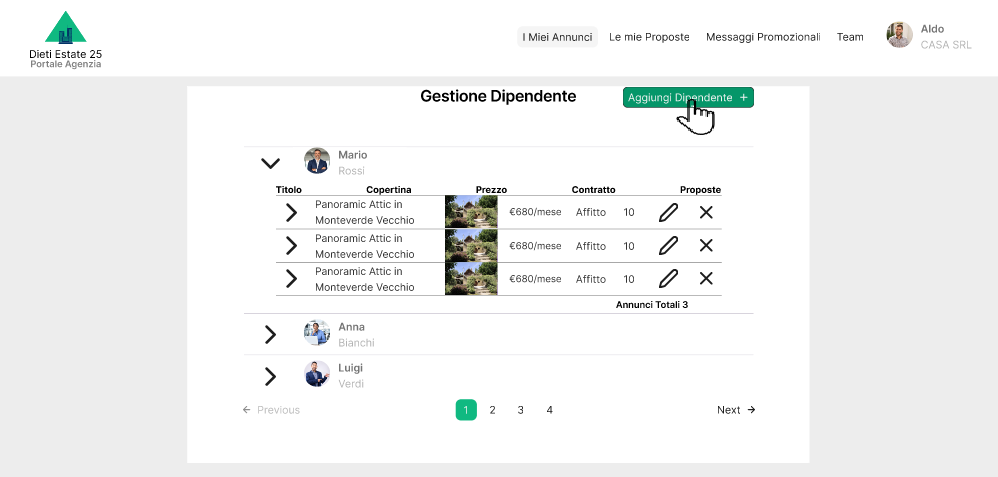
\includegraphics[width=0.7\textwidth]{Immagini/Mockup/nuovoAgente/scenario principale/clickNuovoDipendente.png} \\
				Cockburn: step 1
			\end{tabular}
		};
		
		% Nodo per immagine 2 con didascalia sotto, posizionato a destra di img1
		\node (img2) [below=of img1] {
			\begin{tabular}{c}
				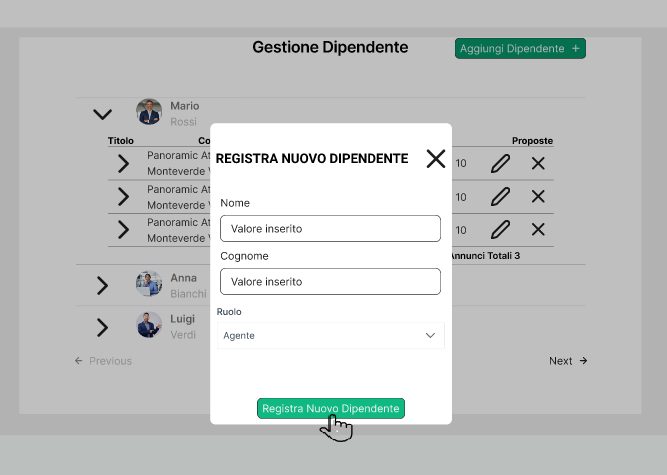
\includegraphics[width=0.7\textwidth]{Immagini/Mockup/nuovoAgente/scenario principale/clickFormNuovoAgente.png} \\
				Cockburn: step 2/3/4
			\end{tabular}
		};
		
		% Nodo per immagine 3 con didascalia sotto, posizionato sotto img2
		\node (img3) [below=of img2] {
			\begin{tabular}{c}
				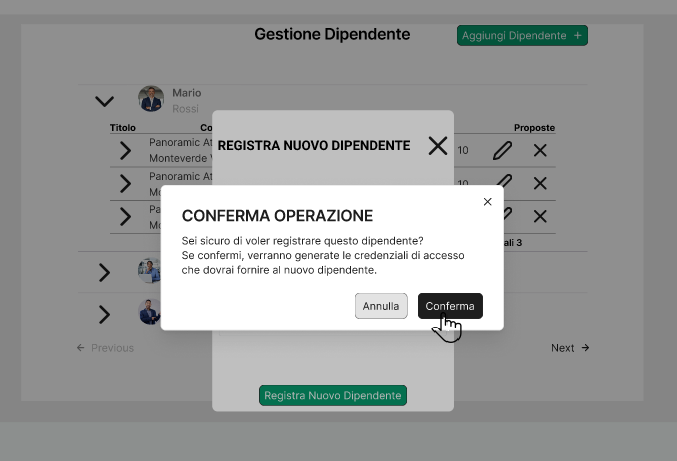
\includegraphics[width=0.7\textwidth]{Immagini/Mockup/nuovoAgente/scenario principale/ClickAllertConferma.png} \\
				Cockburn: step 5/6
			\end{tabular}
		};
		
		% Disegna le frecce
		\draw[->, thick] (img1) -- (img2);
		\draw[->, thick] (img2) -- (img3);
		
	\end{tikzpicture}
	\caption{Mockup: scenario principale della tabella di Cockburn del caso d'uso: Registra nuovo agente.}
	\label{fig:tikz_flow}
\end{figure}

\newpage

\begin{figure}[H]
	\centering
	\begin{tikzpicture}[node distance=1.5cm and 1cm, auto]
		% Nodo per immagine 1 con didascalia sotto
		\node (img1) {
			\begin{tabular}{c}
				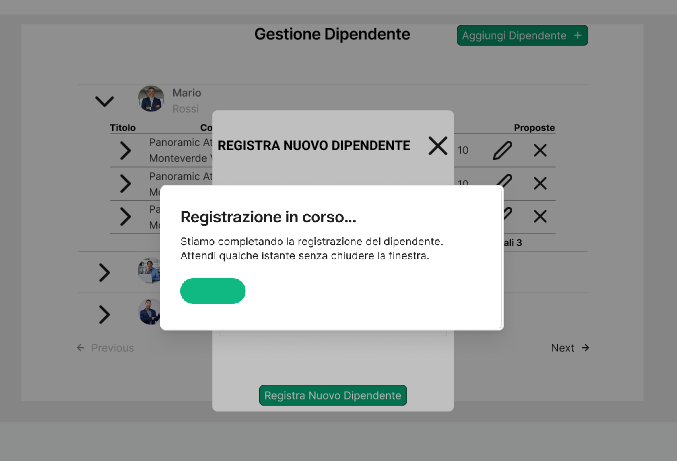
\includegraphics[width=0.7\textwidth]{Immagini/Mockup/nuovoAgente/scenario principale/caricamentoRegistrazione.png} \\
				Cockburn: step 6/7/9
			\end{tabular}
		};
		
		% Nodo per immagine 2 con didascalia sotto, posizionato a destra di img1
		\node (img2) [below=of img1] {
			\begin{tabular}{c}
				\includegraphics[width=0.7\textwidth]{Immagini/Mockup/nuovoAgente/scenario principale/allertRegistrazioneEffettuata.png} \\
				Cockburn: step 10
			\end{tabular}
		};
		
		% Nodo per immagine 3 con didascalia sotto, posizionato sotto img2
		\node (img3) [below=of img2] {
			\begin{tabular}{c}
				\includegraphics[width=0.7\textwidth]{Immagini/Mockup/nuovoAgente/scenario principale/visualizzazioneNuovaRegistrazione.png} \\
				Cockburn: step 11
			\end{tabular}
		};
		
		% Disegna le frecce
		\draw[->, thick] (img1) -- (img2);
		\draw[->, thick] (img2) -- (img3);
		
	\end{tikzpicture}
	\caption{Mockup: scenario principale della tabella di Cockburn del caso d'uso: Registra nuovo agente.}
	\label{fig:tikz_flow}
\end{figure}

\newpage

\subsubsection{Estensione A: Campi Non Compilati o Compilati Erroneamente}

Durante la procedura di registrazione di un nuovo agente, il manager potrebbe tentare di completare l’operazione senza aver inserito tutti i dati richiesti o compilando alcuni campi in modo errato.
Per prevenire errori di input e garantire la coerenza delle informazioni salvate nel sistema, è previsto un controllo di validazione lato client.

\subsubsection{Gestione del Messaggio di Errore}
Nel momento in cui il manager clicca su \textbf{“Registra dipendente”} con uno o più campi incompleti o non validi, il sistema intercetta l’errore e mostra un messaggio specifico sotto ciascun campo non conforme.
Il messaggio indica chiaramente la tipologia di errore (es. campo obbligatorio, formato non valido, valore numerico errato), fornendo un feedback immediato e mirato.

L’interfaccia rimane attiva e consente al manager di correggere i dati direttamente nella stessa schermata, evitando la perdita delle informazioni già inserite.
Una volta completate le correzioni, il manager può ripetere l’operazione di registrazione, tornando così al flusso principale dello scenario (Step 3).

Questa soluzione progettuale segue i principi della \textbf{visibilità dello stato del sistema} e della \textbf{prevenzione degli errori} \cite{nielsen1995}, migliorando la comprensibilità e riducendo la frustrazione dell’utente.

\begin{figure}[H]
	\centering
	\begin{tikzpicture}[node distance=1.5cm and 1cm, auto]
		% Nodo per immagine 1 con didascalia sotto
		\node (img1) {
			\begin{tabular}{c}
				\includegraphics[width=0.7\textwidth]{Immagini/Mockup/nuovoAgente/extension A/nomeNonInserito.png} \\
				Cockburn: step 4.A
			\end{tabular}
		};
		
		% Nodo per immagine 2 con didascalia sotto, posizionato a destra di img1
		\node (img2) [below=of img1] {
			\begin{tabular}{c}
				\includegraphics[width=0.7\textwidth]{Immagini/Mockup/nuovoAgente/extension A/messaggioDiErrore.png} \\
				Cockburn: step 5.A
			\end{tabular}
		};
	
		
		% Disegna le frecce
		\draw[->, thick] (img1) -- (img2);
		
	\end{tikzpicture}
	\caption{Mockup: Extension A della tabella di Cockburn del caso d'uso: Registra nuovo agente.}
	\label{fig:tikz_flow}
\end{figure}



\subsubsection{Estensione B: Nome e Cognome già Registrati}

Nel caso in cui il manager tenti di registrare un agente con nome e cognome già presenti nel sistema, viene eseguito un controllo automatico per evitare la duplicazione dei profili e garantire l’univocità dei dati.

\subsubsection{Gestione del Conflitto e Generazione dell’Email Alternativa}
Dopo aver cliccato su \textbf{“Conferma”}, il sistema mostra una breve fase di caricamento e verifica l’esistenza di un profilo con lo stesso nome e cognome.
In caso di corrispondenza, il sistema genera automaticamente un’email alternativa che include un identificativo univoco, assicurando così la distinzione tra gli utenti.

Completata la procedura, il sistema ritorna al passo 9 dello scenario principale e la registrazione viene finalizzata correttamente.
Questa soluzione applica il principio della \textbf{gestione flessibile degli errori}, consentendo di proseguire l’operazione senza interruzioni e mantenendo la consistenza dei dati.




\subsubsection{Estensione C: Annullamento della Registrazione nella Finestra di Conferma}

Nel caso in cui, all’interno della finestra di conferma, il manager scelga di annullare la registrazione, il sistema interrompe il processo evitando la creazione di un nuovo agente.

\subsubsection{Comportamento del Sistema}
Se il manager clicca su \textbf{“Annulla”} invece di confermare l’operazione, la finestra di dialogo viene chiusa e il flusso ritorna al passo 3 dello scenario principale, consentendo di modificare i dati inseriti o abbandonare la procedura.

Questa interazione segue il principio del \textbf{controllo da parte dell’utente} \cite{nielsen1995}, garantendo la possibilità di interrompere o correggere un’azione prima che diventi definitiva.
\subsubsection{Estensione D: Mancata Connessione al Sistema}

In alcune circostanze, il manager potrebbe non riuscire a completare la registrazione a causa di problemi di connessione o di un temporaneo malfunzionamento del server.
Il sistema gestisce questa evenienza fornendo un chiaro feedback sull’esito negativo dell’operazione.

\subsubsection{Gestione dell’Errore di Connessione}
Dopo aver cliccato su \textbf{“Conferma”}, il sistema mostra un breve stato di caricamento.
Se la connessione al server non riesce, viene visualizzato un pop-up di allerta che informa l’utente dell’impossibilità di completare la registrazione per motivi tecnici.

In questo caso, l’\textbf{use case è considerato fallito}, ma il manager può chiudere il messaggio e riprovare l’operazione una volta ristabilita la connessione.
Questa soluzione si basa sui principi di \textbf{visibilità dello stato del sistema} e di \textbf{recuperabilità dall’errore}, assicurando chiarezza e prevedibilità anche in situazioni di errore tecnico.
\begin{figure}[H]
	\centering
	\begin{tikzpicture}[node distance=1.5cm and 1cm, auto]
			% Nodo per immagine 3 con didascalia sotto, posizionato sotto img2
		\node (img1){
			\begin{tabular}{c}
				\includegraphics[width=0.7\textwidth]{Immagini/Mockup/nuovoAgente/scenario principale/ClickAllertConferma.png} \\
				Cockburn: step 6.D
			\end{tabular}
		};
		
		% Nodo per immagine 1 con didascalia sotto
		\node (img2)  [below=of img1] {
			\begin{tabular}{c}
				\includegraphics[width=0.7\textwidth]{Immagini/Mockup/nuovoAgente/scenario principale/caricamentoRegistrazione.png} \\
				Cockburn: step 7.D
			\end{tabular}
		};
		
		% Nodo per immagine 3 con didascalia sotto, posizionato sotto img2
		\node (img3) [below=of img2] {
			\begin{tabular}{c}
				\includegraphics[width=0.7\textwidth]{Immagini/Mockup/nuovoAgente/extension D/messaggioDiErrore.png} \\
				Cockburn: step 8.D
			\end{tabular}
		};
		
		% Disegna le frecce
		\draw[->, thick] (img1) -- (img2);
		\draw[->, thick] (img2) -- (img3);
		
	\end{tikzpicture}
	\caption{Mockup: Extension D della tabella di Cockburn del caso d'uso: Registra nuovo agente.}
	\label{fig:tikz_flow}
\end{figure}


\clearpage
\newpage
